

The success of a mixed finite element formulation crucially depends on a proper choice of the local interpolations of the velocity and the pressure. 

%........................................................................................
\subsection{The compatibility condition (or LBB condition, or inf-sup condition)} \label{ss:LBBcond}
\index{general}{LBB} \index{general}{Optimal Rate}

\begin{flushright} {\tiny {\color{gray} lbb.tex}} \end{flushright}
%~~~~~~~~~~~~~~~~~~~~~~~~~~~~~~~~~~~~~~~~~~~~~~~~~~~~~~~~~~~~~~~~~~~~~~~~~~~~~~~~~~~~~~~~~~~~~~~~~~

WARNING: I am not comfortable writing about this topic. What follows is a rough attempt at making sense of it.

\hspace{.4cm}

The Lady{\v z}henskaya-Babu{\v s}ka-Brezzi (LBB\footnote{
\url{https://en.wikipedia.org/wiki/Ladyzhenskaya-Babuska-Brezzi_condition}}) condition is a sufficient 
condition for a saddle point problem to have a unique solution.
For saddle point problems coming from the Stokes equations, 
many discretizations are unstable, giving rise to artifacts such as spurious oscillations. 
The LBB condition gives criteria for when a discretization of a saddle point problem is stable. 
It also assures convergence at the optimal rate. 

Bochev \& Gunzburger \cite{bogu09} state: ``
The terminology 'LBB' originates from the facts that this condition was first explicitly discussed
in the finite element setting for saddle point problems by Brezzi\footnote{
\url{https://en.wikipedia.org/wiki/Franco_Brezzi}} \cite{brez74} and that it is a special case of
the general weak-coercivity condition first discussed for finite element methods by Ivo Babu{\v s}ka\footnote{
\url{https://en.wikipedia.org/wiki/Ivo_Babuska}}
\cite{babu71} and that, in the continuous setting of the Stokes equation, this condition was first proved to
hold by Olga Ladyzhenskaya\footnote{\url{https://en.wikipedia.org/wiki/Olga_Ladyzhenskaya}}; see \cite{lady69}.''

Unfortunately, to quote Donea \& Huerta \cite{dohu03}: 
``In the finite element context, it is by no means easy to prove whether or not a given
velocity-pressure pair satisfies the LBB compatibility condition.''
Elman \etal state: ``[...] Choosing spaces for which the discrete inf-sup condition holds
and is a delicate matter, and seemingly natural choices of velocity and pressure approximation
do not work. [...] In general, care must be taken to make the velocity space 
rich enough compared to the pressure space.''

The LBB condition, or inf-sup condition can be proven in different ways, 
and standard techniques have been designed
as listed in Boffi \etal (2008) \cite{bobf08}.

%p129
Elman \etal \cite{elsw} state that ``The inf-sup condition is a sufficient condition 
for the pressure to be unique up to constant in the case of an enclosed flow.''
This can also be proven for other boundary conditions.
This approach, based on the macro-element technique \cite{sten90} is explored in Appendix \ref{app:Gel}.

It can be shown that, provided the kernel (null space) of matrix $\G$ is zero,
the Stokes matrix is non-singular, that is $\vec{\cal V}$ and $\vec{\cal P}$ 
are uniquely defined, and the Schur complement matrix $\SSS$ is positive definite. 
Simply put, taking $\vec{\cal V}=\vec{0}$ in the discretised Stokes system 
without body forces yields $\G \cdot \vec{\cal P}=\vec{0}$ and implies
that any pressure solution is only unique up to the null space of the matrix $\G$.

We know that the Schur complement matrix $\SSS$ is positive definite if and only if all of its eigenvalues are positive.
One could then (numerically) compute the eigenvalues of $\SSS$ and check that these are indeed strictly positive
to show that $\SSS$ is positive definite but that would prove very costly. 

Another way is to see that $\SSS$ is positive definite only if $\text{ker}(\G)=\{0\}$.
Again to quote Donea \& Huerta \cite{dohu03}: ``If this is the case, the partitioned Stokes matrix  
is non-singular and delivers uniquely defined velocity and pressure fields. If this is not the case, a
stable and convergent velocity field might be obtained, but the pressure field is likely
to present spurious and oscillatory results.'' 
Note that in the case of the $Q_1 \times P_0$ element it has been shown that the multiple families of 
checkboard pressure modes actually lie in the kernel of $\G$. \cite{sagl81a,sagl81b}

\hspace{.4cm}

We can look at this in a different manner, as explained in Elman \etal \cite{elsw}:
the unique solvability of the matrix system
\begin{equation}
\left(
\begin{array}{cc}
\K & \G \\
\G^T & 0 
\end{array}
\right)
\cdot 
\left(
\begin{array}{c}
\vec{\cal V} \\ \vec{\cal P}
\end{array}
\right)
=
\left(
\begin{array}{c}
\vec{f} \\ \vec{h}
\end{array}
\right)
\label{eq:lbbsyst}
\end{equation}
is determined by looking at the homogeneous system
\begin{equation}
\left(
\begin{array}{cc}
\K & \G \\
\G^T & 0 
\end{array}
\right)
\cdot 
\left(
\begin{array}{c}
\vec{\cal V} \\ \vec{\cal P}
\end{array}
\right)
=
\left(
\begin{array}{c}
\vec{0} \\ \vec{0}
\end{array}
\right)
\end{equation}
or,
\begin{eqnarray}
\K \cdot \vec{\cal V} + \G \cdot \vec{\cal P} &=& \vec{0} \nn\\
\G^T \cdot \vec{\cal V} &=& \vec{0}
\end{eqnarray}
To start, premultiply the first equation by $\vec{\cal V}^T$ and the second by 
$\vec{\cal P}^T$. The second yields
$\vec{\cal P}^T \cdot \G^T \cdot \vec{\cal V} = ( \vec{\cal V}^T \cdot \G\cdot \vec{\cal P}  )^T = \vec{0}$
which is present in the first equation so that it simplifies to $\vec{\cal V}^T\cdot \K \cdot \vec{\cal V} = \vec{0}$.
Since $\K$ is positive definite, it follows that $\vec{\cal V}=\vec{0}$, implying unique solvability
with respect to the velocity. 

On the other hand, unique solvability with respect to the pressure is problematic. Substituting $\vec{\cal V}=\vec{0}$
in the system above gives $\G \cdot \vec{\cal P} = \vec{0}$, and implies that any pressure solution is only unique 
up to the nullspace of the matrix $\G$. 
The bottom line is that if Eq.~\eqref{eq:lbbsyst} is to properly represent a continuous Stokes
problem, then the mixed approximation spaces need to be chosen carefully.
Specifically, we have to ensure that $null(\G)=\{1\}$ in the case of enclosed flow,
and that $null(\G)=\{0\}$, otherwise.





%........................................................................................
\subsection{Families}
\index{general}{Taylor-Hood}

The family of {\color{olive} Taylor-Hood} finite element spaces on triangular/tetrahedral 
grids is given by ${\bm P}_k \times P_{k-1}$ with $k\geq 2$, 
and on quadrilateral/hexahedral grids by ${\bm Q}_k \times Q_{k-1}$ with $k\geq 2$.
This means that the pressure is then approximated by continuous functions. 

These finite elements are very popular, in particular the pairs for $k=2$, i.e.
${\bm Q}_2\times Q_1$ and ${\bm P}_2\times P_1$.
The reason why $k\geq 2$ comes from the fact that the 
${\bm Q}_1 \times Q_0$ (often referred to as ${\bm Q}_1 \times P_0$) and ${\bm P}_1\times P_0$
are not stable elements (they are not inf-sup stable), as
shown in John \cite[p64]{john16} and \cite[p67]{john16}. 

\begin{remark}
Note that a similar element to ${\bm Q}_2 \times Q_1$ has been proposed
and used succesfully used in \textcite{taho73} (1973) and \textcite{hota74} (1974): 
it is denoted by ${\bm Q}_2^{(8)} \times Q_1$ 
since the center node ('$x^2y^2$') and its associated degrees of freedom have been removed. It 
has also been proved to be LBB stable. These are also called {\color{olive} Serendipity} elements. 
\end{remark}

%........................................................................................
\subsection{The bi/tri-linear velocity - constant pressure element ($Q_1\times P_0$)}
\label{ss:pairq1p0}
\begin{flushright} {\tiny {\color{gray} pair\_q1p0.tex}} \end{flushright}
%~~~~~~~~~~~~~~~~~~~~~~~~~~~~~~~~~~~~~~~~~~~~~~~~~~~~~~~~~~~~~~~~~~~~~~~~~~~~~~~~~~~~~~~~~~~~~~~~~~


\begin{minipage}{0.48\textwidth}
\begin{center}
\begin{flushright} {\tiny {\color{gray} \tt (tikz\_q1p0.tex)}} \end{flushright}
%~~~~~~~~~~~~~~~~~~~~~~~~~~~~~~~~~~~~~~~~~~~~~~~~~~~~~~~~~~~~~~~~~~~~~~~~~~~~~~~~~~~~~~~~~~~~~~~~~~

\begin{tikzpicture}
%\draw[fill=gray!23,gray!23](0,0) rectangle (5,5);
%\draw[step=0.5cm,gray,very thin] (0,0) grid (4,4); %background grid
\draw[thick] (1,1) -- (3,1.2) -- (2.7,3) -- (1.1,3.1) -- cycle;  
\node[] at (0.8,0.8) {0};
\node[] at (3.2,1) {1};
\node[] at (2.9,3.1) {2};
\node[] at (0.9,3.2) {3};
\draw[violet] (1.9,2.075) circle (4pt);
\draw[black,fill=teal] (1,1)   circle (2pt);
\draw[black,fill=teal] (3,1.2)  circle (2pt);
\draw[black,fill=teal] (2.7,3)  circle (2pt);
\draw[black,fill=teal] (1.1,3.1) circle (2pt);
\draw[black,fill=teal] (3.1,0.2) circle (2pt); 
\node[] at (3.4,0.2) {$\vec\upnu$};
\draw[violet] (4.1,0.2) circle (4pt); 
\node[] at (4.4,0.2) {$p$};
\node[] at (2.5,4.5) {4 vel. nodes, 1 press. node};
\end{tikzpicture}

\end{center}
\end{minipage}
\begin{minipage}{0.48\textwidth}
\begin{center}

\begin{tikzpicture}
%\draw[fill=gray!23,gray!23](0,0) rectangle (5,5);
%\draw[step=0.25cm,gray,very thin] (0,0) grid (5,4); %background grid
\draw[thick] (1,0.5) -- (3.25,0.75) -- (3,3) -- (0.5,2.5) -- cycle; %1-2-6-5
\draw[thick] (3.25,0.75) -- (4,1.5) -- (4.25,3.75) -- (3,3) -- cycle; %2-3-7-6
\draw[thick] (0.5,2.5) -- (3,3) -- (4.25,3.75) -- (1.75,3.5) -- cycle; %5-6-7-4
\draw[thin]   (1,0.5) -- (2,1.75) -- (1.75,3.5) -- (0.5,2.5)   --cycle; % 1-0-4-5 
\draw[thin] (2,1.75) -- (4,1.5); 
%\node[] at (0.8,0.8) {0};
%\node[] at (3.2,1) {1};
%\node[] at (2.9,3.1) {2};
%\node[] at (0.9,3.2) {3};
\draw[violet] (2.5,2.) circle (4pt);
\draw[black,fill=teal] (1,0.5)   circle (2pt);
\draw[black,fill=teal] (3.25,0.75)   circle (2pt);
\draw[black,fill=teal] (3,3)   circle (2pt);
\draw[black,fill=teal] (0.5,2.5)   circle (2pt);
\draw[black,fill=teal] (1.75,3.5)  circle (2pt);
\draw[black,fill=teal] (4.25,3.75)  circle (2pt);
\draw[black,fill=teal] (4,1.5) circle (2pt);
\draw[black,fill=teal] (2,1.75) circle (2pt);
\draw[black,fill=teal] (3.1,0.2) circle (2pt); 
\node[] at (3.4,0.2) {$\vec\upnu$};
\draw[violet] (4.1,0.2) circle (4pt); 
\node[] at (4.4,0.2) {$p$};
\node[] at (2.5,4.5) {8 vel. nodes, 1 press. node};
\end{tikzpicture}

\end{center}
\end{minipage}

However simple it may look, the \index{general}{$Q_1 \times P_0$} element is 
one of the hardest elements to analyze and many questions are still open about its properties. 
The element does not satisfy the inf-sup condition \cite[p211]{hugh}. 
In Gresho \& Sani \cite{grsa} it is labeled as follows: slightly unstable but highly usable. 

The $Q_1 \times P_0$ mixed approximation is the lowest order conforming approximation 
method defined on a rectangular grid. It also happens to be the most famous example 
of an unstable mixed approximation method.
\cite[p235]{elsw}.
\textcite{boni84} (1984) and \textcite{boni85} (1985) show that it is not stable.

This element is discussed in Fortin (1981) \cite{fort81}, Fortin \& Fortin (1985) \cite{fofo85} 
and in Pitk\"aranta \& Saarinen (1985) \cite{pisa85} in the context of multigrid use.

This element is plagued by so-called pressure checkerboard modes which
have been thoroughly analysed \cite{grsi94}, \cite{chpc95}, \cite{sagl81a,sagl81b}.
These can be filtered out \cite{chpc95}. Smoothing techniques are also discussed in \cite{legs79}, 
and explained in Section~\ref{psmoothing}.

\Literature: Fortin \& Boivin (1990) \cite{fobo90}, Gresho \& Lee (1985) \cite{grle85},
Le Tallec \& Ruas (1986) \cite{leru86}, Oden \& Jacquotte (1984) \cite{odja84}


%----------------------------------------------------------------------
\subsection{The bi/tri-quadratic velocity - bi/tri-linear pressure element ($Q_2 \times Q_1$)}
\label{ss:pairq2q1}
\begin{flushright} {\tiny {\color{gray} \tt pair\_q2q1.tex}} \end{flushright}
%~~~~~~~~~~~~~~~~~~~~~~~~~~~~~~~~~~~~~~~~~~~~~~~~~~~~~~~~~~~~~~~~~~~~~~~~~~~~~~~~~~~~~~~~~~~~~~~~~~

\noindent
\begin{minipage}{0.48\textwidth}
\begin{center}
\begin{flushright} {\tiny {\color{gray} (tikz\_q2q1.tex)}} \end{flushright}
%~~~~~~~~~~~~~~~~~~~~~~~~~~~~~~~~~~~~~~~~~~~~~~~~~~~~~~~~~~~~~~~~~~~~~~~~~~~~~~~~~~~~~~~~~~~~~~~~~~

%\begin{center}
\begin{tikzpicture}
%\draw[fill=gray!23,gray!23](0,0) rectangle (5,5);
%\draw[step=0.5cm,gray,very thin] (0,0) grid (4,4); %background grid
\draw[thick] (1,1) -- (3,1.2) -- (2.7,3) -- (1.1,3.1) -- cycle;  
\node[] at (0.7,0.8) {0};
\node[] at (3.3,1) {1};
\node[] at (3,3.1) {2};
\node[] at (0.8,3.2) {3};
\draw[black,fill=teal] (1,1)     circle (2pt); \draw[violet] (1,1) circle (4pt);
\draw[black,fill=teal] (3,1.2)   circle (2pt); \draw[violet] (3,1.2) circle (4pt);
\draw[black,fill=teal] (2.7,3)   circle (2pt); \draw[violet] (2.7,3) circle (4pt);
\draw[black,fill=teal] (1.1,3.1) circle (2pt); \draw[violet] (1.1,3.1) circle (4pt);
\draw[black,fill=teal] (2,1.1) circle (2pt) ; \node[] at (2,0.8) {4};
\draw[black,fill=teal] (2.85,2.1) circle (2pt) ; \node[] at (3.1,2.1) {5};
\draw[black,fill=teal] (1.9,3.05) circle (2pt) ; \node[] at (1.9,3.3) {6};
\draw[black,fill=teal] (1.05,2.05) circle (2pt) ; \node[] at (0.8,2) {7};
\draw[black,fill=teal] (1.9,2.075) circle (2pt) ; \node[] at (2.1,2) {8};
\draw[black,fill=teal] (3.1,0.2) circle (2pt); 
\node[] at (3.4,0.2) {$\vec\upnu$};
\draw[violet] (4.1,0.2) circle (4pt); 
\node[] at (4.4,0.2) {$p$};
\node[] at (2.5,4.5) {9 vel. nodes, 4 press. nodes};
\end{tikzpicture}
%\end{center}

\end{center}
\end{minipage}
\hfill
\begin{minipage}{0.48\textwidth}
\begin{center}



%\begin{center}
\begin{tikzpicture}
%\draw[fill=gray!23,gray!23](0,0) rectangle (5,5);
%\draw[step=0.5cm,gray,very thin] (0,0) grid (5,4); %background grid
\draw[thick] (1,0.5) -- (2,0.55) --(3.25,0.75) -- (3,3) -- (0.5,2.5) -- cycle; %1-9-2-6-5
\draw[thick] (3.25,0.75) -- (3.6,1.05) -- (4,1.5) -- (4.25,3.75) -- (3,3) -- cycle; %2-10-3-7-6
\draw[thick] (0.5,2.5) -- (3,3) -- (4.25,3.75) -- (1.75,3.5) -- (1.1,3.1) -- cycle; %5-6-7-4-13
\draw[thin]   (1,0.5) -- (1.5,1.25) -- (2,1.75) -- (1.75,3.5) -- (1.1,3.1) -- (0.5,2.5) --cycle; % 1-8-0-4-5-13 
\draw[thin] (2,1.75) -- (3,1.75) -- (4,1.5); %0-11-3
%pressure nodes
\draw[violet] (2,1.75) circle (4pt); % 0 
\draw[violet] (1,0.5) circle (4pt); % 1 
\draw[violet] (3.25,0.75) circle (4pt); % 2 
\draw[violet] (4,1.5) circle (4pt); % 3 
\draw[violet] (1.75,3.5) circle (4pt); % 4 
\draw[violet] (0.5,2.5) circle (4pt); % 5 
\draw[violet] (3,3) circle (4pt); % 6 
\draw[violet] (4.25,3.75) circle (4pt); % 7 
%velocity nodes
\draw[black,fill=teal] (1,0.5)   circle (2pt);
\draw[black,fill=teal] (3.25,0.75)   circle (2pt);
\draw[black,fill=teal] (3,3)   circle (2pt);
\draw[black,fill=teal] (0.5,2.5)   circle (2pt);
\draw[black,fill=teal] (1.75,3.5)  circle (2pt);
\draw[black,fill=teal] (4.25,3.75)  circle (2pt);
\draw[black,fill=teal] (4,1.5) circle (2pt);
\draw[black,fill=teal] (2,1.75) circle (2pt);
\draw[black,fill=teal] (1.5,1.25) circle (2pt); % 8 
\draw[black,fill=teal] (2,0.55) circle (2pt); % 9 
\draw[black,fill=teal] (3.6,1.05) circle (2pt); % 10
\draw[black,fill=teal] (3,1.75) circle (2pt); % 11
\draw[black,fill=teal] (0.75,1.5) circle (2pt); % 12
\draw[black,fill=teal] (1.1,3.1) circle (2pt); % 13
\draw[black,fill=teal] (0.75,1.5) circle (2pt); % 18
\draw[black,fill=teal] (2.7,1.1) circle (2pt); % 21
\draw[black,fill=teal] (3.6,3.35) circle (2pt); % 21
\draw[black,fill=teal] (3.,3.62) circle (2pt); % 21
\draw[black,fill=teal] (4.12,2.6) circle (2pt); % 21
\draw[black,fill=teal] (1.89,2.5) circle (2pt); % 21
\draw[black,fill=teal] (1.75,2.75) circle (2pt); % 21
\draw[black,fill=teal] (3.12,1.9) circle (2pt); % 21
\draw[black,fill=teal] (3.6,2.2) circle (2pt); % 21
\draw[black,fill=teal] (1.25,2.1) circle (2pt); % 21
\draw[black,fill=teal] (2.4,3.2) circle (2pt); % 21
\draw[black,fill=teal] (2.5,2.5) circle (2pt); % 21

% legend
\draw[black,fill=teal] (3.1,0.2) circle (2pt); \node[] at (3.4,0.2) {$\vec\upnu$};
\draw[violet] (4.1,0.2) circle (4pt); 
\node[] at (4.4,0.2) {$p$};
\node[] at (2.5,4.5) {27 vel. nodes, 8 press. nodes};
\end{tikzpicture}
%\end{center}


\end{center}
\end{minipage}

It belongs to the Taylor-Hood family of elements and satisfies the inf-sup (LBB) condition \cite[p215]{hugh}.
Gresho \& Sani \cite[p554]{grsa} write that in their opinion $div(\vec v)=0$ is not strong enough.
This element, implemented in penalised form, is discussed in Bercovier \& Engelman (1979) \cite{been79} 
and the follow-up paper \cite{been80}. 

It is the default of the \aspect code (see Appendix~\ref{app:codes}).
It is implemented in \stone~18,21,48,91,120,...
 




%----------------------------------------------------------------------
\subsection{The bi/tri-quadratic velocity - discontinuous linear pressure element ($Q_2 \times P_{-1}$)}
\label{ss:pairq2pm1}
\begin{flushright} {\tiny {\color{gray} pair\_q2pm1.tex}} \end{flushright}
%~~~~~~~~~~~~~~~~~~~~~~~~~~~~~~~~~~~~~~~~~~~~~~~~~~~~~~~~~~~~~~~~~~~~~~~~~~~~~~~~~~~~~~~~~~~~~~~~~~

According to \textcite{bobf08} ``This element was apparently discovered 
around a blackboard at the Banff Conference on Finite Elements in Flow Problems (1979)''.

\begin{center}
\begin{flushright} {\tiny {\color{gray} \tt (tikz\_p2pm1.tex)}} \end{flushright}
%~~~~~~~~~~~~~~~~~~~~~~~~~~~~~~~~~~~~~~~~~~~~~~~~~~~~~~~~~~~~~~~~~~~~~~~~~~~~~~~~~~~~~~~~~~~~~~~~~~


%\begin{center}
\begin{tikzpicture}
%\draw[fill=gray!23,gray!23](0,0) rectangle (5,5);
%\draw[step=0.5cm,gray,very thin] (0,0) grid (5,5); %background grid
\draw[thick] (1,1) -- (4,1) -- (4,3) -- (1,3) -- cycle;  
\node[] at (0.7,0.8)  {0};
\node[] at (4.3,0.8)  {1};
\node[] at (4.25,3.1) {2};
\node[] at (0.8,3.2)  {3};
\node[] at (2.5,0.75) {4};
\node[] at (4.3,2)    {5};
\node[] at (2.5,3.25) {6};
\node[] at (0.7,2)    {7};
\node[] at (2.25,1.85){8};

\draw[black,fill=teal] (1,1)   circle (2pt); 
\draw[black,fill=teal] (4,1)   circle (2pt); 
\draw[black,fill=teal] (4,3)   circle (2pt); 
\draw[black,fill=teal] (1,3)   circle (2pt); 
\draw[black,fill=teal] (2.5,1) circle (2pt); 
\draw[black,fill=teal] (2.5,3) circle (2pt); 
\draw[black,fill=teal] (1,2)   circle (2pt); 
\draw[black,fill=teal] (4,2)   circle (2pt); 
\draw[black,fill=teal] (2.5,2) circle (2pt); 

\draw[violet] (2.5,2) circle (4pt);
\draw[violet] (3,2) circle (4pt);
\draw[violet] (2.5,2.5) circle (4pt);

\draw[black,fill=teal] (3.1,0.2) circle (2pt); 
\node[] at (3.4,0.2) {$\vec\upnu$};
\draw[violet] (4.1,0.2) circle (4pt); 
\node[] at (4.4,0.2) {$p$};
\node[] at (2.5,3.85) {9 vel. nodes, 3 press. nodes};
\end{tikzpicture}
%\end{center}

\end{center}

This element is crowned "probably the most accurate 2D element" 
in \textcite{grsa}.

It is characterised by piecewise Biquadratic velocities, 
and piecewise linear discontinuous polynomial pressure. 
The element satisfies the inf-sup condition, see page 211 of \textcite{hugh}, or 
p138 of \textcite{elsw}.
It is used in \textcite{vavs89} (1989) for steady laminar flow in a curved tube. 

See \textcite{boga02} (2002) 
for the two possible choices for the two definitions of the pressure space (mapped and un-mapped), 
and check \stone~76 for their implementation.
\textcite{bobf08} state: ``On a general quadrilateral mesh, the [pressure] space 
can be defined in two different ways: either [it] 
consists of (discontinuous) piecewise linear functions, or it is built
by considering three linear shape functions on the reference unit square and mapping
them to the general elements like it is usually done for continuous finite elements. [...]
We shall refer to the first possibility as unmapped pressure approach and to the
second one as mapped pressure approach.''
Furthermore they state ``So far, we have shown that either the unmapped and the mapped pressure 
approach gives rise to a stable $Q_2\times P_{-1}$ scheme. However, as a consequence of the
results proved in \textcite{arbf02} (2002), we have that the mapped pressure approach cannot achieve 
optimal approximation order. Namely, the unmapped pressure space provides a second-order convergence 
in $L_2$, while the mapped one achieves only ${\cal O}(h)$ in the same norm.''
See also discussion about mapped/unmapped in \textcite{bobf13}.

This element is mentioned in \textcite{kaus10} (2010) and \textcite{pefc89} (1989) 
and it is used in \textcite{freh14} (2014) to study 3D fold growth rates 
(see online supplementary material) and in \textcite{schm08} (2008).

Note that the serendipity version of this pair, i.e. $Q_2^{(20)}\times P_{-1}$ is also LBB stable
as shown in p180 of Reddy \cite{reddybook2}.


%\begin{minipage}{0.58\textwidth}
%\end{minipage}
%\hfill
%\begin{minipage}{0.38\textwidth}
%\end{minipage}




%----------------------------------------------------------------------
\subsection{The biquadratic velocity - discontinuous bilinear pressure element ($Q_2 \times Q_{-1}$)}
\label{ss:pair_q2qm1}

This element is shown in Table~3.13-2 of Gresho \& Sani's book \cite{grsa}, 
and discussed in Section~3.13.6b of the book too. It is {\it not} LBB stable
and has one chequerboard pressure mode.

Used in \textcite{grsu02} (2002) and compared with $Q_1\times P_0$, $Q_2\times P_{-1}$ and 
$Q_2\times Q_1$ for thermal cavity problem with NS equations.


%----------------------------------------------------------------------
\subsection{The stabilised bi/tri-linear velocity - constant pressure element ($Q_1\times P_0$-stab)}
\label{ss:pairq1p0stab}
\begin{flushright} {\tiny {\color{gray} pair\_q1p0stab.tex}} \end{flushright}
%~~~~~~~~~~~~~~~~~~~~~~~~~~~~~~~~~~~~~~~~~~~~~~~~~~~~~~~~~~~~~~~~~~~~~~~~~~~~~~~~~~~~~~~~~~~~~~~~~~

Import from ELEFANT manual!

\Literature: \cite{sike90,vibo92,kesi92,qizh07,lisi12,chco01,chri02}



%--------------------------------------------------------------------------------------------------
\subsection{The stabilised bi/tri-linear velocity - bi/tri-linear pressure element ($Q_1\times Q_1$-stab)}
\label{ss:pairq1q1stab}
\begin{flushright} {\tiny {\color{gray} pair\_q1q1stab.tex}} \end{flushright}
%~~~~~~~~~~~~~~~~~~~~~~~~~~~~~~~~~~~~~~~~~~~~~~~~~~~~~~~~~~~~~~~~~~~~~~~~~~~~~~~~~~~~~~~~~~~~~~~~~~

\begin{minipage}[t]{0.5\textwidth}
\input{tikz/tikz_q1q1}
\end{minipage}
\begin{minipage}[t]{0.5\textwidth}
\input{tikz/tikz_q1q1_3D}
\end{minipage}

See \cite{nosi01} for a fourier analysis of the normal and stablised (a la \cite{hufb86}) $Q_1-Q_1$ element.
This element is used in \cite{bugs09,busa13} in conjunction with AMR. 
Stabilisation is worked out out in \cite{dobo04,bodg06,bodo06}.

$Q_1\times P_0$-stab. Pro: stabilisation can be switched off; Con: stabilisation for deformed elements? 
problem near boundaries: incomplete stencil? choice of parameter $\beta$.

$Q_1\times Q_1$-stab. Pro: easier to implement than $Q_1\times P_0$-stab, stabilisation local to element, easier when elements are not rectangular, no free parameter; Con: stabilisation cannot be switched off.

\Literature: \cite{shry78,temr92,tezd92,grcc95,idsn95,knto00,fros07,lihc09}. See Braack \& Lube \cite{brlu09}
for a review of local projection stabilisation for incompressible flow problems. 

This unstable pair is also used in ice sheet modelling \cite{heah18,zhjg11,zwgg07}
A $P_1\times P_1$ version of it is used in \cite{kahp20}.



%-----------------------------------------------------------------
\subsection{The Rannacher-Turek element - rotated ${ Q}_1\times P_0$} \label{ss:RTq1p0}

\index{general}{$\tilde{Q}_1\times P_0$}
\index{general}{Korn's inequality}
\index{general}{Rannacher-Turek element}
\index{general}{Nonconforming element}

This element is the natural quadrilateral analogue
of the well-known triangular $P_1^{nc} $Stokes element of Crouzeix-Raviart \cite{crra73}.
This element is sometimes called ${\bm Q}_1^{rot} \times Q_0$ or the Rannacher-Turek element 
\cite[Section 3.6.5]{john16} (see also Appendix~B.4, example B.53 of \textcite{john16}).
This rectangular nonconforming \cite{crfa89} element is termed the rotated ${\bm Q}_1$ element 
because of the fact that $r^2-s^2$ can be generated from $rs$ (occurring in the bilinear $Q_1$ 
element) by a rotation of 45$\degree$ \cite[p93]{chen}.
The velocity approximation is achieved by rotated dim-linear functions that have 
continuous degrees of freedom on
the faces of the mesh cells as we have seen in Section~\ref{ss:rq1}.
This element was introduced in Rannacher \& Turek (1992) \cite{ratu92} 
has been proven to satisfy the inf-sup condition. It has been studied comprehensively in Schieweck 
(1997)\footnote{Habilitation thesis in German}, \cite{shzh06} and in Turek \cite{ture94,ture96}.
Superconvergence properties have also been reported \cite{misx06,misx07}.
It has been used in 2D \cite{maky17} and 3D \cite{klll96,gekm08} and forms the basis of the FeatFlow 
software\footnote{\url{http://www.featflow.de/en/index.html}}. 
It is used in the PhD thesis of Gastaldo \cite{gast07} and Ouazzi \cite{ouaz05}.
It has been 
successfully coupled to multigrid solvers \cite{chos98,tuos02}.
This element has been compared to the stabilised ${\bm Q}_1\times P_0$ element \cite{lisi13}.
It is mentioned in \cite{hans11}

It essentially comes in two flavours, the Middle Point (MP) and the Mid Value (MV) one.

\begin{remark} 
John \cite{john16} explains that: "For the point-value-oriented non-conforming finite element spaces (MP), 
the value of the Dirichlet boundary
condition in the barycenter of the faces at the boundary is taken. Using the mean-
value-oriented spaces (MV), one computes the integrals of the boundary condition on
these faces and normalizes with the area of the faces to set the boundary values.
In the case of homogeneous Dirichlet boundary conditions, the boundary values
computed in both ways are zero."
\end{remark}

\begin{remark} 
John also makes a very important point: "There are also unmapped (non-parametric) versions of 
these finite element spaces, which define the polynomials directly on the mesh cell K. It is shown in Rannacher
and Turek (1992) \cite{ratu92} that these versions are inf-sup stable on more general meshes than
the mapped (parametric) version of the ${\bm Q}_1^{rot}\times Q_0$ finite element, e.g., on strongly
nonuniform meshes. Considering all four types of ${\bm Q}_1^{rot}\times Q_0$ finite elements, the
optimal order of convergence on perturbed meshes is achieved only by the mean-
value-oriented version of the unmapped ${\bm Q}_1^{rot}\times Q_0$   finite element.
\end{remark}

Mahmood \etal \cite{maky17} mention a very important fact: "The chosen nonconforming element requires
additional stabilization for handling the deformation tensor formulation due to missing Korn's inequality 
\cite{horg95,knob00,bren04}.
To this end we employ the standard edge oriented stabilization \cite{tuos02,tuou07} in our simulations."
This is a rather unfortunate fact that although LBB stable this element needs an additional 
term in the weak form (see Turek \etal (2002) \cite{tuos02}) 
so as to suppress parasitic velocity modes when the div-grad formulation 
of the Stokes equation is used (as opposed to the Laplace formulation -- see \cite[Section 6.5.2]{dohu03}).

This element is used in \textcite{hala01} (2001) in the context of near incompressible elasticity. 
It is mentioned that it does not fulfill the discrete Korn's inequality. It is then stabilised 
in a discontinuous Galerkin framework.

\Literature \textcite{shee20} (2020), \textcite{chen92} (1992) , \textcite{chen93} (1993) 

\url{https://defelement.com/elements/rannacher-turek.html}






%------------------------------------------------------------------
\subsection{The ${ P}_1\times P_0$ pair} \label{ss:p1p0}
\index{general}{$P_1\times P_0$}
\begin{flushright} {\tiny {\color{gray} \tt  pair\_p1p0.tex}} \end{flushright}
%~~~~~~~~~~~~~~~~~~~~~~~~~~~~~~~~~~~~~~~~~~~~~~~~~~~~~~~~~~~~~~~~~~~~~~~~~~~~~~~~~~~~~~~~~~~~~~~~~~





Elman Silvester Wathen say (5.3.3) that 
\begin{displayquote}
{\color{darkgray}
It can be readily stabilized using the pressure jump
stabilization together with an appropriate macroelement subdivision.}
\end{displayquote}
See \textcite{nosi98} (1998) for globally and locally stabilised versions. 

\textcite{qizh07b} (2007) state: 
\begin{displayquote}
{\color{darkgray}
The element is unstable for any mesh since
the dimension of the discrete velocity space is always less than that of the pressure space (with
Dirichlet boundary condition).
However, this element provides optimal approximations for both
the velocity and the pressure on many mesh families.} 
\end{displayquote}

\begin{center}
\includegraphics[width=12cm]{images/pair_p1p0/qizh07}\\
{\captionfont A crisscross, a Powell–Sabin, a Powell–Sabin–Heindl and a type-2 grid.
Taken from \cite{qizh07}.}
\end{center}

\textcite{arno93} (1993) states: 
\begin{displayquote}
{\color{darkgray}
Unfortunately, this simplest possible Stokes element is notoriously unstable. On any 
triangulation with at least three vertices on the boundary the dimension of the pressure
space exceeds that of the velocity space [...] and the finite
dimensional problem is singular. 
Moreover, while the discrete velocity field $u_h$ is uniquely
determined (as it is for any conforming method for the Stokes problem), for this choice of
elements $u_h$ belongs to the space of divergence-free fields piecewise linear fields, and on
many meshes, for example on a uniform diagonal mesh of the square [...],
this space is known to reduce to zero. So even after accounting for the indeterminancy of
the pressure we have no convergence.}
\end{displayquote}

Example 3.2 of \textcite{bobf08} (2008) explains neatly the locking phenomenon and how 
to circumvent it via a so-called cross-grid macroelement. See also 
\textcite{hokl03} (2003).

In his lecture notes\footnote{\url{https://www.math.tamu.edu/~guermond/}}, 
Guermond states 
\begin{displayquote}
{\color{darkgray}
A simple alternative to the 
$Q_1\times P_0$ element consists of using the $P_1\times P_0$ element.
Let ${\cal T}_h$  be a mesh of $D$ composed of affine simplices, and approximate the 
velocity with continuous piecewise linear polynomials and the pressure with
(discontinuous) piecewise constants. Since the velocity is piecewise linear, its
divergence is constant on each simplex. As a result, testing the divergence
of the velocity with piecewise constants enforces the divergence to be zero
everywhere. That is to say, the $P_1\times P_0$ finite element yields a velocity 
approximation that is exactly divergence-free [...]. Unfortunately,
this pair does not satisfy the inf-sup condition.}
\end{displayquote}

I have not found a paper yet which showcases its accuracy on a manufactured solution
and compares it to other element pairs.


CHECK example 3.70 in \textcite{john16} (book),


%------------------------------------------------------------------
\subsection{The ${ P}_2\times P_0$ pair} \label{ss:p2p0}
\begin{flushright} {\tiny {\color{gray} \tt  pair\_p2p0.tex}} \end{flushright}
%~~~~~~~~~~~~~~~~~~~~~~~~~~~~~~~~~~~~~~~~~~~~~~~~~~~~~~~~~~~~~~~~~~~~~~~~~~~~~~~~~~~~~~~~~~~~~~~~~~

 \cite{bobf08}, \cite{cakp18} stable (Kanschat book)

compared with P1NC-P0 and BR element in \textcite{cakp15} (2015).


%------------------------------------------------------------------
\subsection{The ${ Q}_2\times Q_0$ pair} \label{ss:pairq2q0}
\index{general}{${\bm Q}_2 \times Q_0$}

Quadratic velocities, constant pressure. The element satisfies the inf-sup condition, 
but the constant pressure assumption may require fine discretisation.
source?


%------------------------------------------------------------------
\subsection{The ${ P}_1\times P_1$-stabilised pair} \label{ss:P1P1stab}

Like its quadrilateral counterpart ${\bm Q}_1\times Q_1$, the 
$P_1\times P_1$ pair is not stable and needs to be stabilised \cite{nosi98,tasu00}.
TerraNeo code uses stabilised with PSPG \cite{babd20}.

\textcite{nosi98}

%--------------------------------------------------------------------------------------------------
\subsection{The ${ P}_1^+\times P_1$ (MINI) pair in 2D \& 3D \label{pair:mini}}
\begin{flushright} {\tiny {\color{gray} pair\_mini.tex}} \end{flushright}
%~~~~~~~~~~~~~~~~~~~~~~~~~~~~~~~~~~~~~~~~~~~~~~~~~~~~~~~~~~~~~~~~~~~~~~~~~~~~~~~~~~~~~~~~~~~~~~~~~~

\noindent
\begin{minipage}{0.48\textwidth}
The \index{general}{MINI element} MINI element was first introduced in 
\textcite{arbf84} (1984).
It is also discussed in Section~3.6.1 of \textcite{john16} (2016) and in Section~6.1 
of \textcite{bobf08} (2008). It is thoroughly studied in \textcite{cibo19} (2019).

As explained in Braess \cite{braess}, since the support of the cubic bubble is restricted to the element, 
the associated variable (dofs living on the bubble) can be eliminated from the resulting 
system of linear equations by static condensation. \index{general}{Static Condensation}
Also, the MINI element is cheaper than the Taylor-Hood element but it is commonly accepted
that it yields a poorer approximation of the pressure.
\end{minipage}\hfill
\begin{minipage}{0.48\textwidth}
\input{tikz/tikz_mini}
\end{minipage}

\begin{remark}
Note that \textcite{frol03} (2003) propose an equal-order-linear-continuous 
velocity-pressure variables which is enriched 
with velocity {\it and} pressure bubble functions to model the Stokes problem. 
They show by static condensation that
these bubble functions give rise to a stabilized method involving least-squares forms of 
the momentum and of the
continuity equations. In some cases their approach recovers 
the MINI element. Also check \textcite{gamt08} (2008).
\end{remark}

The 3D MINI element is not very common but it is used for instance in \textcite{pico98} (1998) or
\textcite{tokv09} (2009). 
It is also said to be LBB stable in Reddy \cite[p180]{reddybook2}.
It is used in \cite{furstoss} phd thesis in the context of microstructures deformation modeling, 
which itself cites \textcite{camb13} (2013).

\begin{center}
\includegraphics[width=8cm]{images/mini/mini3D}\\
{\captionfont Velocity and pressure nodes for the 3D MINI element, taken from \cite{pico98}}
\end{center}

Note that this element is used in Braess \& Wriggers (2000) \cite{brwr00} 
in the context of Arbitrary Lagrangian Eulerian 
finite element analysis of free surface flows, and also 
in \textcite{zldf07} (2007) for subduction with X-FEM technique. 
\index{general}{X-FEM}. It is also mentioned in \textcite{nath93} (1993).

The 2D element is implemented in \stone~\ref{f120}.


%--------------------------------------------------------------------------------------------------
\subsection{The ${ P}_2\times P_1$ pair \label{ss:p2p1}}
\begin{flushright} {\tiny {\color{gray} pair\_p2p1.tex}} \end{flushright}
%~~~~~~~~~~~~~~~~~~~~~~~~~~~~~~~~~~~~~~~~~~~~~~~~~~~~~~~~~~~~~~~~~~~~~~~~~~~~~~~~~~~~~~~~~~~~~~~~~~

\noindent
\begin{minipage}{0.54\textwidth}
From Segal \cite{segal}: \say{Taylor-Hood elements \cite{taho73} 
are characterized by the fact that the pressure is continuous in the region $\Omega$. 
A typical example is the quadratic triangle (${\bm P}_2\times P_1$ element).
In this element the velocity is approximated by a quadratic polynomial and the pressure by a
linear polynomial. One can easily verify that both approximations are continuous over 
the element boundaries.}

It can be shown, Segal (1979), that this element is admissible if at least 3 elements 
are used. The quadrilateral counterpart of this triangle is the ${\bm Q}_2\times Q_1$ element.
Reddy and Gartling \cite[p179]{reddybook2} also report this element to be LBB stable.
It is also mentioned in \textcite{nath93}.

\Literature: Schubert \& Anderson \cite{scan85}, Leng \etal \cite{lejx14}, Cuffaro \etal \cite{cump20}
\end{minipage}
\hfill
\begin{minipage}{0.42\textwidth}
\begin{center}
\begin{flushright} {\tiny {\color{gray} (tikz\_p2p1.tex)}} \end{flushright}
%~~~~~~~~~~~~~~~~~~~~~~~~~~~~~~~~~~~~~~~~~~~~~~~~~~~~~~~~~~~~~~~~~~~~~~~~~~~~~~~~~~~~~~~~~~~~~~~~~~

%\begin{center}
\begin{tikzpicture}
%\draw[fill=gray!23,gray!23](0,0) rectangle (5,5);
%\draw[step=0.5cm,gray,very thin] (0,0) grid (5,3.5); %background grid
\draw[thick] (1,0.5) -- (4,1)  -- (3,3) -- cycle; %1-9-2-6-5

%pressure nodes
\draw[violet] (1,0.5) circle (4pt); % 0 
\draw[violet] (4,1) circle (4pt); % 1 
\draw[violet] (3,3) circle (4pt); % 2 

%velocity nodes
\draw[black,fill=teal] (1,0.5)   circle (2pt);
\draw[black,fill=teal] (4,1)   circle (2pt);
\draw[black,fill=teal] (3,3)   circle (2pt);

\draw[black,fill=teal] (2.5,0.75)   circle (2pt);
\draw[black,fill=teal] (2,1.75)   circle (2pt);
\draw[black,fill=teal] (3.5,2)   circle (2pt);

% legend
\draw[black,fill=teal] (3.1,0.2) circle (2pt); \node[] at (3.4,0.2) {$\vec\upnu$};
\draw[violet] (4.1,0.2) circle (4pt); 
\node[] at (4.4,0.2) {$p$};
\node[] at (2.5,3.75) {6 vel. nodes, 3 press. nodes};
\end{tikzpicture}
%\end{center}


\end{center}
\end{minipage}






%----------------------------------------------------------------------
\subsection{The ${ P}_2^+\times P_{-1}$ pair  (Crouzeix-Raviart) }
\label{sec:crouzeix-raviart}
\begin{flushright} {\tiny {\color{gray} pair\_crouzeixraviart.tex}} \end{flushright}
%~~~~~~~~~~~~~~~~~~~~~~~~~~~~~~~~~~~~~~~~~~~~~~~~~~~~~~~~~~~~~~~~~~~~~~~~~~~~~~~~~~~~~~~~~~~~~~~~~~

Since the $P_2\times P_{-1}$ pair is not LBB stable \cite[p179]{reddybook2}, 
it is enhanced by a cubic bubble and is therefore called $P_2^+\times P_{-1}$. 

This element was first introduced in \cite{crra73}.
It is the element used in the MILAMIN code \cite{daks08}.
It is a seven-node triangle with quadratic velocity shape 
functions enhanced by a cubic bubble function and discontinuous linear interpolation for 
the pressure field \cite{cuss86}. 
This element is LBB stable and no additional stabilization techniques are required\cite{elsw}.
The '+' in its name stands for the bubble while the '-' stands for the discontinuous
character of the pressure field: once again, it is $P_1$ over the element, but discontinuous
across element edges.

\begin{remark}
Cuvelier \etal, 1986 \cite{cuss86} recommend a 6-point or 7-point quadrature rule for this element.
\end{remark}

\begin{remark}
Segal \cite{segal} explains 
for output purposes (printing, plotting etc.) the discontinuous pressures are averaged 
in vertices for all the adjoining elements. See also Fig. 7.3 of \cite{cuss86}.
\end{remark}

\begin{remark}
The simplest Crouzeix-Raviart element is the non-conforming linear triangle 
with constant pressure ($P_1\times P_0$) \cite{cuss86}. 
\end{remark}

It is worth noting that this element has more degrees of freedom  than the 
Taylor-Hood element for the same order of accuracy. However, since the 
bubble can be eliminated, one can design a modified version of this element.
\todo[inline]{Check Cuvelier book chapter 8 for modified element}


\begin{remark}
I have once asked the (main) author of MILAMIN why he chose this element, for 
example over the $P_2\times P_1$. His answer is as follows:
"Elements with continuous pressure  are incapable of converging in the Linf 
norm for mechanical problems exhibiting pressure jumps such as the inclusion-host setup. 
During my MSc and PhD I was focusing on sharp heterogeneities, so this is why I decided 
to choose $P_2^+\times P_{-1}$. 
You will see that it is also easy to invert the pressure mass matrix for such elements, 
which is really useful (both for the augmentation and preconditioning)."
\end{remark}

This element is used by Poliakov and Podlachikov \cite{popo92} to study the deformation of the surface above a rising diapir. Note that they actually use a "13 point integration formula (Hughes
1987) for calculation of the stiffness matrix was used in order
t o conserve detailed information from the marker field in
the coarse FEM mesh". 
It is also used in \cite{anmp15} in the context of a new free-surface stabilization scheme. 
It is the element used in LaCoDe \cite{demh19}.



%----------------------------------------------------------------------
\subsection{The ${ P}_2^+\times P_{1}$ pair \label{ss:p2pp1}}

This element pair is not to be mistaken for the Crouzeix-Raviart. Both share the same $P_2^+$ space
for the velocity but this element has a continuous linear pressure.  
It is mentioned in Table~3.13-1 of \textcite{grsa}: ``LBB stable. Second order. cubic bubble. good element''.
It is also mentioned in \textcite{sofo87} (1987).

Implemented in \stone~120.


%------------------------------------------------------------------
\subsection{The ${ P}_2\times (P_1+P_0)$ pair} \label{ss:p2p1p0}


This element pair is discussed in 5.3.3 of Elman, Silvester and Wathen: 

``[Another] possibility is to construct a hybrid pressure approximation by 
combining the continuous linear pressure approximation with the discontinuous constant pres-
sure approximation. The resulting mixed method is referred to as the $P_2-P_{-1*}$ 
approximation and enjoys the best of both worlds; it has locally 
incompressibility, and yet it does not have its accuracy compromised by
the lower order pressure [of $P_2\times P_0$]. 
Perhaps surprisingly, this element is also uniformly stable.'' 

\begin{center}
\includegraphics[width=7cm]{images/pair_p2p1p0/elsw}\\
{\captionfont Taken from \textcite{elsw}.}
\end{center}

In Gresho \& Sani table 3.13-1: ``LBB stable yes. Better than P2P1, element mass balance.
more work than P2P1. 2 hydrostatic modes. Second order.'' 
Note that they call it P2(P1+P0) and that they call the CR element P2+P1 (not P-1) so that 
I don't know whether its pressure is continuous or not. However since they state 'element mass balance'
it probably means disc pressure. On the other hand, the drawing and legend of this element in the table 
is clear: pressure at the 3 vertices is continuous and there is a cross (disc pressure) in the middle. 

\begin{center}
\includegraphics[width=4cm]{images/pair_p2p1p0/grsa2}
\includegraphics[width=12cm]{images/pair_p2p1p0/grsa1}\\
{\captionfont Taken from \textcite{grsa}.}
\end{center}

\textcite{bocg12} (2012) state: ``[...] the pressure space $Q_h$ is defined as the sum of two finite 
element spaces, namely $P_k+P_0$ ($k \ge d- 1$) [...]for the enhanced Hood–Taylor [...]. 
However, it can be easily observed that the sum is not direct, 
since globally constant functions can be represented exactly by means of piecewise 
$P_0$ or continuous $P_k$ ($k \ge 1$) elements.
Concerning the implementation of the method, we avoid the computation of the basis
functions of such a finite element by testing the discrete problem (2.3) with the basis 
functions of the two subspaces separately. By the above discussion it turns out that the resulting
matrix is rank-deficient, with kernel of dimension 1.''




%------------------------------------------------------------------
\subsection{The ${ Q}_2\times (Q_1+Q_0)$ pair} \label{ss:q2q1q0}
It is a rather peculiar element pair (triplet?). The velocity space is the standard $Q_2$ space
but the pressure space is the sum of two spaces, i.e. $Q_1$ {\it and} $Q_0$.
Please see Section~\ref{ss:p2p1p0} on the $P_2\times (P_1+P_0)$ element.

\begin{center}
\includegraphics[width=9cm]{images/pair_q2q1q0}\\
{\captionfont Taken from \textcite{grsa}'s book.}
\end{center}

It is implemented in \stone~120.


%------------------------------------------------------------------
\subsection{The ${ P}_3\times P_2$ pair} \label{ss:p3p2}

$P_3\times P_2$ mentioned in \cite{sten90}   \index{general}{$P_3\times P_2 element$}

See \stone~120


%------------------------------------------------------------------
\subsection{The Raviart-Thomas family} \label{ss:raviart_thomas}
\begin{flushright} {\tiny {\color{gray} \tt pair\_raviart\_thomas.tex}} \end{flushright}
%~~~~~~~~~~~~~~~~~~~~~~~~~~~~~~~~~~~~~~~~~~~~~~~~~~~~~~~~~~~~~~~~~~~~~~~~~~~~~~~~~~~~~~~~~~~~~~~~~~
 
In \textcite{hald03} (2003) we find: 
\begin{displayquote}
{\color{darkgray}
$P_1^\perp \times P_0$ symbol denotes an element with 
normal velocity nodes in the middle of each edge of the
triangulation [...]. This element, also called low order Raviart–Thomas element 
(Raviart and Thomas, 1977), is based on flux conservation on elements edges and 
the resulting scheme is very close to a finite volume scheme.
}
\end{displayquote}

It is mentioned in \textcite{john16}, appendix B.3, example B.45: 
\begin{displayquote}
{\color{darkgray}
the normal component of v 
on each face is a constant. The normal component of functions from RT0 is
continuous across faces of the mesh cells.
}
\end{displayquote}


In \textcite{chen93a} (1993) we read:
\begin{displayquote}
{\color{darkgray}
Arnold and Brezzi [2] showed, for
example, that the Raviart-Thomas mixed method of lowest order is
equivalent to the usual $P_1$-nonconforming method modified by augmenting
the classical $P_1$-nonconforming space with $P_3$-bubbles and then proved that
the equivalence is useful not only for implementing the mixed method but
also for deriving error estimates.
}
\end{displayquote}


There is an entry on Wikipedia\footnote{\url{
https://en.wikipedia.org/wiki/Raviart-Thomas_basis_functions
}} but it is short and not so useful, except for
\begin{displayquote}
{\color{darkgray}
In applied mathematics, Raviart–Thomas basis functions are vector basis functions used 
in finite element and boundary element methods. They are regularly used as basis 
functions when working in electromagnetics. 
}
\end{displayquote}

There is also a useful entry on Stackexchange\footnote{\url{
https://scicomp.stackexchange.com/questions/20245/raviart-thomas-elements-on-reference-square}}:
\begin{displayquote}
{\color{darkgray}
There are quadrilateral Raviart-Thomas elements. 
In two dimensions, the polynomial space for $RT_k$ is given by 
$P_{k+1,k} \times P_{k,k+1}$, where
\[
P_{k,l}=\left\{ \sum_{i=0}^{k} \sum_{j=0}^{l} a_{ij} x^i y^j: a_{ij}\in \R  \right\}
\]

A typical polynomial for $k=0$ would thus be 
\[
\left(
\begin{array}{c}
a_1+b_1 x \\
a_2+b_2 y
\end{array}
\right)
\]
and for $k=1$:
\[
\left(
\begin{array}{c}
a_1+b_1 x +c_1x^2 +d_1 y + e_1 xy  + f_2 x^2 y\\
a_2+b_2 y +c_2y^2 +d_2 x + e_2 xy  + f_2 x y^2
\end{array}
\right)
\]
Hence, $dim(RT_1)=12$, and in general, $dim(RT_k)=2(k+1)(k+2)$. 
This means you need two additional degrees of freedom, which should be located on the 
interior of the element. (In general, for $RT_k$ you take $k+1$ normal derivatives on each facet, 
and the remaining degrees of freedom from the interior.)

For Raviart-Thomas elements, you usually take moments rather than 
point evaluations, i.e., the remaining conditions come from the conditions 
\[
\int_{-1}^{+1} \int_{-1}^{+1} \phi_i(x,y)q_j(x,y)dx dy = \delta_{ij}
\]
where the ${q_j}$ are a basis of $P_{k-1,k}\times P_{k,k-1}$ (e.g. $1,x,y$ for $k=1$).
To make it easier to get a full nodal basis, the facet degrees of freedom are 
usually not taken as point evaluation, but also as moment conditions: 
\[
\int_{e_m} \phi_i(s)^T \nu_{e_m} q_{m,j}(s) ds
\]
where $e_m$ is one of the four edges, $\nu_{e_m}$ is the corresponding outer normal, 
and for each $m$, the $q_{m,j}$ form a basis of $P_k(e_m)$ (e.g. {1,x} or {1,y}
for $k=1$ depending on the edge orientation).
Together, these degrees of freedom are unisolvent (i.e., the corresponding system 
of basis functions is always invertible).
}
\end{displayquote}




- Raviart Thomas 0 RT0 \cite{rath77} ? mentioned/defined/drawn in 4.2.2 of 
Kanschat book. Also exist for quads see 4.2.37

-Check \textcite{brfo}



This element is implemented in deal.ii and we 
read\footnote{\url{https://www.dealii.org/current/doxygen/deal.II/classFE__RaviartThomas.html}}:
\begin{displayquote}
{\color{darkgray}
The Raviart-Thomas space is designed to solve problems in which the solution only 
lives in the space $H^{div}=\{ {\bm u} \in L_2 :div({\bm u}) \in L_2\}$, 
rather than in the more commonly used space $H^1=\{ {\bm u} \in L_2 : \nabla {\bm u} \in L_2 \}$. 
In other words, the solution must be a vector field whose divergence is square integrable, 
but for which the gradient may not be square integrable. The typical application for this space 
(and these elements) is to the mixed formulation of the Laplace equation and related situations, 
see for example step-20. The defining characteristic of functions in  $H^{div}$ is that they are 
in general discontinuous - but that if you draw a line in 2d (or a surface in 3d), 
then the normal component of the vector field must be continuous across the line (or surface) 
even though the tangential component may not be. As a consequence, the Raviart-Thomas element 
is constructed in such a way that (i) it is vector-valued, (ii) the shape functions are 
discontinuous, but (iii) the normal component of the vector field represented by each shape 
function is continuous across the faces of cells.

Other properties of the Raviart-Thomas element are that 
(i) it is not a primitive element ; 
(ii) the shape functions are defined so that certain integrals over the faces are 
either zero or one, rather than the common case of certain point values being 
either zero or one. 

We follow the commonly used - though confusing - definition of the ``degree'' of RT elements. 
Specifically, the ``degree'' of the element denotes the polynomial degree of the 
largest complete polynomial subspace contained in the finite element space, 
even if the space may contain shape functions of higher polynomial degree. 
The lowest order element is consequently FE\_RaviartThomas(0), i.e., 
the Raviart-Thomas element ``of degree zero'', even though the functions of this space 
are in general polynomials of degree one in each variable. This choice of ``degree'' 
implies that the approximation order of the function itself is degree+1, as with usual polynomial spaces. 
}
\end{displayquote}

On the defelement site\footnote{\url{https://defelement.com/elements/raviart-thomas.html}} we find 
that it is defined on triangles, tetrahedra, quadilaterals and hexahedra.
with the number of dofs defined as follows:
\begin{itemize}
\item triangle: $k(k+2)$
\item tetrahedron: $k(k+1)(k+3)/2$
\item quadrilateral: $2k(k+1)$
\item hexahedron: $3k^2(k+1)$
\end{itemize}



\noindent
\underline{\bf Degree 1 Raviart–Thomas on a triangle - Lagrange variant}

\begin{center}
\includegraphics[width=3cm]{images/pair_raviart-thomas/element-Raviart-Thomas-variant-equispaced-triangle-1-dofs-large}\\
{\captionfont Taken from \url{https://defelement.com/}}
\end{center}

${\cal V}$ is a finite dimensional polynomial space on of dimension $n$ and is spanned by 
\[
\left( \begin{array}{c}1 \\ 0  \end{array} \right),
\left( \begin{array}{c}0 \\ 1  \end{array} \right),
\left( \begin{array}{c}x \\ y  \end{array} \right)
\]
Functionals and basis functions:

\begin{center}
\includegraphics[width=3cm]{images/pair_raviart-thomas/element-Raviart-Thomas-variant-equispaced-triangle-1-0-large}
\includegraphics[width=3.3cm]{images/pair_raviart-thomas/element-Raviart-Thomas-variant-equispaced-triangle-1-1-large}
\includegraphics[width=3cm]{images/pair_raviart-thomas/element-Raviart-Thomas-variant-equispaced-triangle-1-2-large}\\
{\captionfont Taken from \url{https://defelement.com/}}
\end{center}

\[
l_0: {\bm v} \rightarrow \int_{e_0} {\bm v} \cdot (1) \hat{n}_0
\]
\[
l_1: {\bm v} \rightarrow \int_{e_1} {\bm v} \cdot (1) \hat{n}_1
\]
\[
l_2: {\bm v} \rightarrow \int_{e_2} {\bm v} \cdot (1) \hat{n}_2
\]
where $e_0$ is the 0th edge and $\hat{n}_0$ is the normal to facet 0,
where $e_1$ is the 1st edge and $\hat{n}_1$ is the normal to facet 1,
where $e_2$ is the 2nd edge and $\hat{n}_2$ is the normal to facet 2.

We have then
\[
{\bm \phi}_0 = \left( \begin{array}{c} -x\\-y  \end{array} \right)
\qquad
{\bm \phi}_1 = \left( \begin{array}{c} x-1\\y  \end{array} \right)
\qquad
{\bm \phi}_2 = \left( \begin{array}{c} -x \\ 1-y  \end{array} \right)
\]
These DOFs are associated with edge 0,1,2 of the reference element.




%-------------------------------------------------------------------------
\noindent
\underline{\bf Degree 1 Raviart–Thomas on a quadrilateral - Lagrange variant}

\begin{center}
\includegraphics[width=3cm]{images/pair_raviart-thomas/element-NCF-variant-equispaced-quadrilateral-1-dofs}\\
{\captionfont Taken from \url{https://defelement.com/}}
\end{center}

${\cal V}$ is a finite dimensional polynomial space on of dimension $n$ and is spanned by 
\[
\left( \begin{array}{c}1 \\ 0  \end{array} \right),
\left( \begin{array}{c}0 \\ 1  \end{array} \right),
\left( \begin{array}{c}x \\ 0  \end{array} \right),
\left( \begin{array}{c}0 \\ y  \end{array} \right)
\]

Functionals and basis functions:

\begin{center}
\includegraphics[width=3cm]{images/pair_raviart-thomas/element-NCF-variant-equispaced-quadrilateral-1-0}
\includegraphics[width=3.5cm]{images/pair_raviart-thomas/element-NCF-variant-equispaced-quadrilateral-1-1}
\includegraphics[width=3cm]{images/pair_raviart-thomas/element-NCF-variant-equispaced-quadrilateral-1-2}
\includegraphics[width=3cm]{images/pair_raviart-thomas/element-NCF-variant-equispaced-quadrilateral-1-3}\\
{\captionfont Taken from \url{https://defelement.com/}}
\end{center}


\[
l_0: {\bm v} \rightarrow \int_{e_0} {\bm v} \cdot (1) \hat{n}_0
\]
\[
l_1: {\bm v} \rightarrow \int_{e_1} {\bm v} \cdot (1) \hat{n}_1
\]
\[
l_2: {\bm v} \rightarrow \int_{e_2} {\bm v} \cdot (1) \hat{n}_2
\]
\[
l_3: {\bm v} \rightarrow \int_{e_3} {\bm v} \cdot (1) \hat{n}_3
\]


where $e_0$ is the 0th edge and $\hat{n}_0$ is the normal to facet 0,
where $e_1$ is the 1st edge and $\hat{n}_1$ is the normal to facet 1,
where $e_2$ is the 2nd edge and $\hat{n}_2$ is the normal to facet 2,
where $e_3$ is the 4th edge and $\hat{n}_3$ is the normal to facet 3.


We have then
\[
{\bm \phi}_0 = \left( \begin{array}{c} 0 \\ 1-y  \end{array} \right)
\qquad
{\bm \phi}_1 = \left( \begin{array}{c} x-1 \\0  \end{array} \right)
\qquad
{\bm \phi}_2 = \left( \begin{array}{c} -x \\ 0  \end{array} \right)
\qquad
{\bm \phi}_2 = \left( \begin{array}{c} 0 \\y  \end{array} \right)
\]
These DOFs are associated with edge 0,1,2 of the reference element.

----------------------------------------

\fullcite{arbf05}




%------------------------------------------------------------------
\subsection{The Bernaudi-Raugel pair} \label{ss:bernaudi_raugel}

- from \textcite{cakp15}: The BR-FEM after Bernardi and Raugel \cite{bera85} is a modification of the P2P0 - FEM.
It is sometimes also called reduced $P_2\times P_0$ -FEM \cite{cakp15}

\textcite{bera85} (1985); 

\textcite{cakp15} (2015) state that this element also exists in 3D.

\includegraphics[width=5cm]{images/pair_bernardi_raugel/cakp15}

It is also mentioned in \textcite{bobf13} although it seems it is there called the SMALL element (p474).

In Lederer: "Consider the case d = 2. Above exam-
ple shows, that we only need to control the normal velocity at the edge, i.e. adding the
edge bubble for both components of the velocity seems to be sub optimal (with respect to
computational costs and the expected approximation properties). The idea now is to only
add the normal edge bubble."




%------------------------------------------------------------------
\subsection{The Scott-Vogelius pair} \label{ss:scott_vogelius}
\index{general}{Scott-Vogelius pair}
\begin{flushright} {\tiny {\color{gray} \tt pair\_scott\_vogelius.tex}} \end{flushright}
%~~~~~~~~~~~~~~~~~~~~~~~~~~~~~~~~~~~~~~~~~~~~~~~~~~~~~~~~~~~~~~~~~~~~~~~~~~~~~~~~~~~~~~~~~~~~~~~~~~

It originates in \fullcite{scvo85} (1985). 

 
In Remark 9 (p.29) of \textcite{aubb17} (2017) we find: 
\begin{displayquote}
{\color{darkgray}
We also remark that the discontinuous
pressure version of the Hood–Taylor element typically
results in an unstable method. However, stability can be
recovered by imposing certain restrictions on the mesh for
$k \ge 3$ (see \cite{voge83}; \cite{scvo85}), or
by taking advantage of suitable stabilization procedures for
$k\ge 1$ (see Mansfield, 1982; Boffi, 1995).
}
\end{displayquote}

In \textcite{fams21} (2021) we find:
\begin{displayquote}
{\color{darkgray}
The Scott-Vogelius element is given by choosing continuous piecewise 
polynomials of degree $k$ for the velocity and discontinuous piecewise 
polynomials of degree $k-1$ for the pressure. While this clearly
implies that $\nabla\cdot V_h \in Q_h$, inf-sup stability of the 
Scott–Vogelius element is more delicate, and is a topic of ongoing research. 
In two dimensions, Scott \& Vogelius proved \cite{scvo85} that the element is inf-sup
stable for $k\ge 4$ if the mesh does not have nearly singular vertices. 
In three dimensions, it was proven more recently in \cite{zhan11b} 
that the element is stable for $k\ge 6$ on uniform meshes. The stability on general
tetrahedral meshes continues to be an open question.

On barycentrically refined meshes, however, the pair is known to 
be stable for polynomial order
$k = d$, see [48, Section 4.6] for the 2D case and 
\cite{zhan05} for the 3D case. If one is willing to 
consider the more complicated Powell–Sabin split, the order 
can be reduced further to $k=d-1$ \cite{zhan08,zhan11a}. The two
refinement patterns are shown for the two dimensional case 
in Figure 1 [see below]. In this work we will consider
the case of $k \ge d$ on barycentrically refined meshes, but 
the arguments apply mutatis mutandis to the Powell–Sabin split.
}
\end{displayquote}

\begin{center}
\includegraphics[width=9cm]{images/pair_scott_vogelius/scottvogelius_split}\\
{\captionfont 
Barycentrically refined triangle (also known as Alfeld split) on the left,
and Powell–Sabin split on the right.\\ Taken from \textcite{fams21} (2021).}
\end{center}

\index{general}{Powell-Sabin}

\textcite{cael11} (2011) state:
\begin{displayquote}
{\color{darkgray}
The SV element pair is not yet very well known,
and so we now give a brief description of it. In essence, the SV pair is the same as
the Taylor-Hood pair except that the pressure space is discontinuous and either
(i) for $k \ge d$, the mesh is a barycenter refinement of a regular mesh, or
(ii) for $k = 2, d = 3$, the mesh is formed from a barycenter refined mesh by
connecting the barycenter nodes (i.e., a Powell–Sabin tetrahedralization).
In short, polynomials of degree $k$ and $k-1$ are used to approximate the velocity
and pressure spaces, respectively, and the mesh ${\cal T}_h$ that is used must be derived from
a regular triangulation (tetrahedralization) of $\Omega$, where each element is refined as
stated above. With these mesh constructions, it was proved by Zhang in [42, 44] that
the SV elements are LBB stable, and, consequently, also have optimal approximation
properties. It is well known that the TH pair is LBB stable and admits optimal
approximation properties for these cases as well [9]. We will restrict our definition of
SV elements to these cases where they are LBB stable.
}
\end{displayquote}

On page 112 of \textcite{john16} we read:
\begin{displayquote}
{\color{darkgray}
The Scott–Vogelius finite element considers still $P_k/P^{disc}_{k-1}$, $k \ge d$, 
but on special meshes, which allow to show the satisfaction of the 
discrete inf-sup condition.
[...]
This pair of finite element spaces $P_k/P^{disc}_{k-1}$
are weakly divergence-free, which is a desirable property.
[...]
The fulfillment of the discrete inf-sup condition 
was proved already in \textcite{scvo85} (1985) in the two-dimensional 
case for $k\ge 4$ if there is no so-called singular vertex in the mesh.
An internal vertex is said to be singular if edges which meet at the vertex fall onto
two straight lines.

The basic idea to overcome this problem consists in using meshes 
without singular vertices. To this end, so-called barycentric-refined 
grids are constructed. Starting from any admissible triangular mesh, 
new edges are introduced by connecting all
vertices of a mesh cell with the barycenter of this mesh cell. 
This step creates smaller triangles.
On barycentric-refined meshes, the $P_k/P^{disc}_{k-1}$, $k=2,3$ 
pair of finite element spaces was shown to satisfy the discrete inf-sup
condition in Qin's phd thesis (1994). [...]

The use of the $P_2/P^{disc}_{1}$ pair of finite element spaces 
on barycentric-refined meshes can be found occasionally in the literature,
in particular to demonstrate the advantages of using pairs of finite element 
spaces which provide weakly divergence-free velocity solutions, 
e.g. see \textcite{john15} and refs therein.

}
\end{displayquote}


\begin{center}
\includegraphics[width=6cm]{images/pair_scott_vogelius/john16}\\
{\captionfont Barycentric-refined simplicial grid on the unit square}
\end{center}

I hereafter present my own internal numbering for the mesh above (used in \stone~120 for example).
The quadrilateral has been cut once along a diagonal, and then an Alfeld split is used, thereby 
dividing the square in 6 triangles:

\begin{flushright} {\tiny {\color{gray} (tikz\_sv.tex)}} \end{flushright}
%~~~~~~~~~~~~~~~~~~~~~~~~~~~~~~~~~~~~~~~~~~~~~~~~~~~~~~~~~~~~~~~~~~~~~~~~~~~~~~~~~~~~~~~~~~~~~~~~~~


\begin{center} 
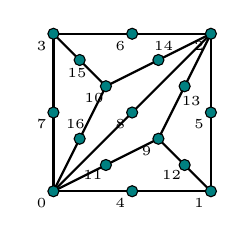
\begin{tikzpicture} 

%\draw[fill=gray!23,gray!23](0,0) rectangle (2.5,2.5);
%\draw[step=0.5cm,gray,very thin] (0,0) grid (2.5,2.5); %background grid

%ielx=1,iely=1,low
\draw[thick] (0,0)--(1.33333,0.66667);
\draw[thick] (2,0)--(1.33333,0.66667);
\draw[thick] (2,2)--(1.33333,0.66667);
%ielx=1,iely=1,high
\draw[thick] (0,0)--(0.666667,1.3333);
\draw[thick] (0,2)--(0.666667,1.3333);
\draw[thick] (2,2)--(0.666667,1.3333);

\draw[thick] (0,0) -- (2,0) -- (2,2) -- (0,2) -- cycle; 
\draw[thick] (0,0) -- (2,2) ; %diag


%\draw[thick] (6,0) -- (4,2) -- (6,4) ; 
\draw[black,fill=teal] ( 0.000000 , 0.000000)     circle (2pt); 
\node[] at ( -0.150000, -0.150000 ) {\tiny 0 }; 
\draw[black,fill=teal] ( 2.000000 , 0.000000)     circle (2pt); 
\node[] at ( 1.850000, -0.150000 ) {\tiny 1 }; 
\draw[black,fill=teal] ( 2.000000 , 2.000000)     circle (2pt); 
\node[] at ( 1.850000, 1.850000 ) {\tiny 2 }; 
\draw[black,fill=teal] ( 0.000000 , 2.000000)     circle (2pt); 
\node[] at ( -0.150000, 1.850000 ) {\tiny 3 }; 
\draw[black,fill=teal] ( 1.000000 , 0.000000)     circle (2pt); 
\node[] at ( 0.850000, -0.150000 ) {\tiny 4 }; 
\draw[black,fill=teal] ( 2.000000 , 1.000000)     circle (2pt); 
\node[] at ( 1.850000, 0.850000 ) {\tiny 5 }; 
\draw[black,fill=teal] ( 1.000000 , 2.000000)     circle (2pt); 
\node[] at ( 0.850000, 1.850000 ) {\tiny 6 }; 
\draw[black,fill=teal] ( 0.000000 , 1.000000)     circle (2pt); 
\node[] at ( -0.150000, 0.850000 ) {\tiny 7 }; 
\draw[black,fill=teal] ( 1.000000 , 1.000000)     circle (2pt); 
\node[] at ( 0.850000, 0.850000 ) {\tiny 8 }; 
\draw[black,fill=teal] ( 1.333333 , 0.666667)     circle (2pt); 
\node[] at ( 1.183333, 0.516667 ) {\tiny 9 }; 
\draw[black,fill=teal] ( 0.666667 , 1.333333)     circle (2pt); 
\node[] at ( 0.516667, 1.183333 ) {\tiny 10 }; 
\draw[black,fill=teal] ( 0.666667 , 0.3333)     circle (2pt); 
\node[] at ( 0.5, 0.2 ) {\tiny 11 }; 
\draw[black,fill=teal] ( 1.6667 , 0.3333)     circle (2pt); 
\node[] at ( 1.5, 0.2 ) {\tiny 12 }; 
\draw[black,fill=teal] ( 1.6667 , 1.3333)     circle (2pt); 
\node[] at ( 1.75, 1.15 ) {\tiny 13 }; 
\draw[black,fill=teal] ( 0.3333,0.666667)     circle (2pt); 
\node[] at ( 1.4,1.85 ) {\tiny 14}; 
\draw[black,fill=teal] ( 0.3333, 1.6667)     circle (2pt); 
\node[] at ( 0.3,1.5 ) {\tiny 15 }; 
\draw[black,fill=teal] ( 1.3333, 1.6667)     circle (2pt); 
\node[] at ( 0.28,0.85 ) {\tiny 16 }; 


\end{tikzpicture} 
%\end{center} 


%\begin{center} 
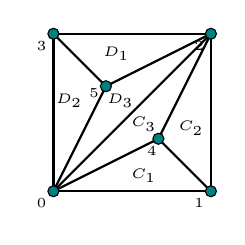
\begin{tikzpicture} 

%\draw[fill=gray!23,gray!23](0,0) rectangle (2.5,2.5);
%\draw[step=0.5cm,gray,very thin] (0,0) grid (2.5,2.5); %background grid

%ielx=1,iely=1,low
\draw[thick] (0,0)--(1.33333,0.66667);
\draw[thick] (2,0)--(1.33333,0.66667);
\draw[thick] (2,2)--(1.33333,0.66667);
%ielx=1,iely=1,high
\draw[thick] (0,0)--(0.666667,1.3333);
\draw[thick] (0,2)--(0.666667,1.3333);
\draw[thick] (2,2)--(0.666667,1.3333);

\draw[thick] (0,0) -- (2,0) -- (2,2) -- (0,2) -- cycle; 
\draw[thick] (0,0) -- (2,2) ; %diag

%\draw[thick] (6,0) -- (4,2) -- (6,4) ; 
\draw[black,fill=teal] ( 0.000000 , 0.000000)     circle (2pt); 
\node[] at ( -0.150000, -0.150000 ) {\tiny 0 }; 
\draw[black,fill=teal] ( 2.000000 , 0.000000)     circle (2pt); 
\node[] at ( 1.850000, -0.150000 ) {\tiny 1 }; 
\draw[black,fill=teal] ( 0.000000 , 2.000000)     circle (2pt); 
\node[] at ( -0.150000, 1.850000 ) {\tiny 3 }; 
\draw[black,fill=teal] ( 2.000000 , 2.000000)     circle (2pt); 
\node[] at ( 1.850000, 1.850000 ) {\tiny 2 }; 
\draw[black,fill=teal] ( 1.333333 , 0.666667)     circle (2pt); 
\node[] at ( 1.25, 0.516667 ) {\tiny 4 }; 
\draw[black,fill=teal] ( 0.666667 , 1.333333)     circle (2pt); 
\node[] at ( 0.516667, 1.25 ) {\tiny 5 }; 

\node[] at ( 1.15,0.2 ) {\tiny $C_1$ }; 
\node[] at ( 1.75,0.8 ) {\tiny $C_2$ }; 
\node[] at ( 1.15,0.85 ) {\tiny $C_3$ }; 

\node[] at ( 0.8,1.75 ) {\tiny $D_1$ }; 
\node[] at ( 0.2,1.15 ) {\tiny $D_2$ }; 
\node[] at ( 0.85,1.15 ) {\tiny $D_3$ }; 

\end{tikzpicture} 
\end{center} 



See also \textcite{jolm17} (2017) in which the $P_2\times P_1$, Scott-Vogelius ($P_2\times P_{-1}$), 
Bernardi-Raugel, and $P_2^+\times P_{-1}$ elements 
are compared for a thermo-mechanically driven convection problem in a triangle (see \stone~51, 
although I use the $P_1^+\times P_1$ element in this stone).


\begin{center}
\includegraphics[width=10cm]{images/pair_scott_vogelius/john_scott_vogelius}\\
\captionfont{Taken from John \cite[p70]{john16}.} 
\end{center}


In \textcite{befh21} (2021) this element is used in its 
$(P_3)^2-P_2^{\text{disc}}$ form.

Note that some have proposed to use an incenter-based refinement instead of
a barycenter refinement since it lead to less pronounced aspect ratios\footnote{
The Scott-Vogelius Method for Stokes Problem on Anisotropic Meshes, K Kean, M Neilan, M Schneier,
\url{https://doi.org/10.48550/arXiv.2109.14780}}.
In geometry, the incenter of a triangle is a triangle center, a point defined for 
any triangle in a way that is independent of the triangle's placement or scale. 
The incenter may be equivalently defined as the point where the internal angle bisectors 
of the triangle cross or as the point equidistant from the triangle's sides.

Given the coordinates of the three vertices of a triangle ABC,
the coordinates of the incenter O are
\[
x_O=\frac{ax_A+bx_B+cx_C}{a+b+c}
\qquad
y_O=\frac{ay_A+by_B+cy_C}{a+b+c}
\] 
where $a$, $b$ and $c$ are the side lengths opposite vertex A, B and C.

 


\begin{center}
\url{https://defelement.com/elements/scott-vogelius.html}
\end{center}




%------------------------------------------------------------------
\subsection{The BDM (Brezzi-Douglas-Marini) pair} \label{ss:bdm}
\index{general}{BDM element}
\index{general}{BDM element}
\begin{flushright} {\tiny {\color{gray} \tt  pair\_bdm.tex}} \end{flushright}
%~~~~~~~~~~~~~~~~~~~~~~~~~~~~~~~~~~~~~~~~~~~~~~~~~~~~~~~~~~~~~~~~~~~~~~~~~~~~~~~~~~~~~~~~~~~~~~~~~~

This element is mentioned in Kanschat book \cite{kanschat}, section 4.2.14. 
It also exists for quads see section 4.2.39 in the same book.
It is mentioned in \textcite{chen93a} (1993), also check the book by \textcite{brfo}.
It is well described in \textcite{kanschat17}.
There is an entire chapter (14) of \textcite{ergu21_72} dedicated to H(div) and 
section 14.5.1 to BDM elements. 
Check section 4.1.1 of \cite{aubb17} for triangles and quads.

\begin{center}
\url{https://defelement.com/elements/brezzi-douglas-marini.html}
\end{center}

\begin{itemize}
%++++++++++++++++++++++++++++++++++++++++++++++
\item In \textcite{lomw12} we read:

The Brezzi-Douglas-Marini element was introduced by Brezzi, Douglas and Marini in two dimensions 
(for triangles) in \textcite{brdm85} (1985). The element can be viewed as an alternative to the
Raviart-Thomas element using a complete polynomial space. It was later extended to three 
dimensions (tetrahedra, prisms and cubes) in \textcite{nede86} (1986) 
and \textcite{brdd87} (1987). The definition given
here is based on that of \textcite{nede86} (1986).

The Brezzi-Douglas-Marini element was introduced for mixed formulations of second-order elliptic 
equations. However, it is also useful for weakly symmetric discretizations of the elastic stress
tensor; see Farhloul and Fortin (1997); Arnold et al. (2007).

\begin{center}
\includegraphics[width=8cm]{images/pair_bdm/bdm_lomw12}\\
{\captionfont Taken from \cite{lomw12}. }
\end{center}

The dimension of $BDM_q$ is $(q+1)(q+2)$ for a triangle and $\frac12(q+1)(q+2)(q+3)$
for a tetrahedron.

Check book for definition.

A slight modification of the Brezzi-Douglas-Marini element constrains the element space ${\cal V}$ by
only allowing normal components on the boundary of polynomial degree $q-1$ (rather than the full
polynomial degree $q$). Such an element was suggested on rectangles by \textcite{brdf87} (1987), and the
triangular analogue was given in \textcite{brfo}. In similar spirit, elements with differing
degrees on the boundary suitable for varying the polynomial degree between triangles were derived
in \textcite{brdm85b} (1985).

%++++++++++++++++++++++++++++++++++++++++++++++
\item On the defelement website\footnote{\url{https://defelement.org/elements/brezzi-douglas-marini.html}}
we find a lot of information. Note that the mapping is set to 'contravariant Piola'. 
\todo[inline]{I still need to understand and write about this!}
It belongs to the categories 'Vector-valued elements', and 'H(div) conforming elements'

\begin{center}
% -------------------------------------------------------
% This plot is from DefElement (https://defelement.org)
% and is available under a Creative Commons Attribution
% 4.0 International (CC BY 4.0) license:
% https://creativecommons.org/licenses/by/4.0/
% -------------------------------------------------------
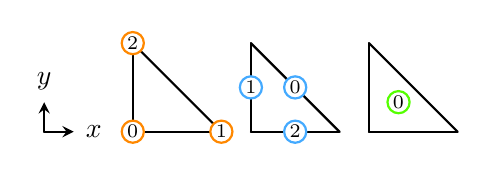
\begin{tikzpicture}[x=1cm,y=1cm]
\definecolor{customcolor0}{HTML}{000000}
\definecolor{customcolor1}{HTML}{44AAFF}
\definecolor{customcolor2}{HTML}{AAAAAA}
\definecolor{customcolor3}{HTML}{DD2299}
\definecolor{customcolor4}{HTML}{FFFFFF}
\definecolor{customcolor5}{HTML}{FF8800}
\definecolor{customcolor6}{HTML}{55FF00}
\draw[-stealth,customcolor0,line width=0.8pt,line cap=round] (25.0,25.0) -- (25.375,25.0);
\draw[-stealth,customcolor0,line width=0.8pt,line cap=round] (25.0,25.0) -- (25.0,25.375);
\node[customcolor0,anchor=west] at (25.405,25.0) {$x$};\node[customcolor0,anchor=south] at (25.0,25.405) {$y$};\draw[customcolor0,line width=0.8pt,line cap=round] (27.25,25.0) -- (26.125,26.125);
\draw[customcolor0,line width=0.8pt,line cap=round] (26.125,25.0) -- (26.125,26.125);
\draw[customcolor0,line width=0.8pt,line cap=round] (26.125,25.0) -- (27.25,25.0);
\draw[customcolor5,line width=0.8pt,fill=customcolor4] (26.125,25.0) circle (4.0pt);
\node[customcolor0,anchor=center] at (26.125,25.0) {\scriptsize 0};\draw[customcolor5,line width=0.8pt,fill=customcolor4] (27.25,25.0) circle (4.0pt);
\node[customcolor0,anchor=center] at (27.25,25.0) {\scriptsize 1};\draw[customcolor5,line width=0.8pt,fill=customcolor4] (26.125,26.125) circle (4.0pt);
\node[customcolor0,anchor=center] at (26.125,26.125) {\scriptsize 2};\draw[customcolor0,line width=0.8pt,line cap=round] (28.75,25.0) -- (27.625,26.125);
\draw[customcolor1,line width=0.8pt,fill=customcolor4] (28.1875,25.5625) circle (4.0pt);
\node[customcolor0,anchor=center] at (28.1875,25.5625) {\scriptsize 0};\draw[customcolor0,line width=0.8pt,line cap=round] (27.625,25.0) -- (27.625,26.125);
\draw[customcolor1,line width=0.8pt,fill=customcolor4] (27.625,25.5625) circle (4.0pt);
\node[customcolor0,anchor=center] at (27.625,25.5625) {\scriptsize 1};\draw[customcolor0,line width=0.8pt,line cap=round] (27.625,25.0) -- (28.75,25.0);
\draw[customcolor1,line width=0.8pt,fill=customcolor4] (28.1875,25.0) circle (4.0pt);
\node[customcolor0,anchor=center] at (28.1875,25.0) {\scriptsize 2};\draw[customcolor6,line width=0.8pt,fill=customcolor4] (29.5,25.375) circle (4.0pt);
\node[customcolor0,anchor=center] at (29.5,25.375) {\scriptsize 0};\draw[customcolor0,line width=0.8pt,line cap=round] (30.25,25.0) -- (29.125,26.125);
\draw[customcolor0,line width=0.8pt,line cap=round] (29.125,25.0) -- (29.125,26.125);
\draw[customcolor0,line width=0.8pt,line cap=round] (29.125,25.0) -- (30.25,25.0);
\end{tikzpicture}
\\
{\captionfont Taken from DefElement \url{https://defelement.org/img/ref-triangle.html}. I have altered 
the font size. Orange: nodes; Blue: edges.}
\end{center}


I reproduce below the figures and basis functions pertaining to the Degree 1 triangle, 
but the site also shows Degree 2 triangle, Degree 1 \& 2 tetrahedron, and so-called 
Lagrange variants.

\begin{center}
\includegraphics[width=3cm]{images/pair_bdm/element-Brezzi-Douglas-Marini-variant-equispaced-triangle-1-dofs}
\includegraphics[width=3cm]{images/pair_bdm/element-Brezzi-Douglas-Marini-variant-equispaced-triangle-1-0}
\includegraphics[width=3cm]{images/pair_bdm/element-Brezzi-Douglas-Marini-variant-equispaced-triangle-1-1}
\includegraphics[width=3cm]{images/pair_bdm/element-Brezzi-Douglas-Marini-variant-equispaced-triangle-1-2}\\
\includegraphics[width=3cm]{images/pair_bdm/element-Brezzi-Douglas-Marini-variant-equispaced-triangle-1-3}
\includegraphics[width=3cm]{images/pair_bdm/element-Brezzi-Douglas-Marini-variant-equispaced-triangle-1-4}
\includegraphics[width=3cm]{images/pair_bdm/element-Brezzi-Douglas-Marini-variant-equispaced-triangle-1-5}\\
{\captionfont Pink: degrees of freedom.}
\end{center}


${\cal V}$ is spanned by 
\[
\left(\begin{array}{c}
1 \\ 0
\end{array}\right),
\left(\begin{array}{c}
0 \\ 1
\end{array}\right),
\left(\begin{array}{c}
x \\ 0
\end{array}\right),
\left(\begin{array}{c}
0 \\ x
\end{array}\right),
\left(\begin{array}{c}
y \\ 0
\end{array}\right),
\left(\begin{array}{c}
0 \\ y
\end{array}\right)
\]
with 
\begin{itemize}
\item DOF \#0 is associated with edge 0 of the reference element with $\vec{\bN}_0$ basis function.
\item DOF \#1 is associated with edge 0 of the reference element with $\vec{\bN}_1$ basis function.
\item DOF \#2 is associated with edge 1 of the reference element with $\vec{\bN}_2$ basis function.
\item DOF \#3 is associated with edge 1 of the reference element with $\vec{\bN}_3$ basis function.
\item DOF \#4 is associated with edge 2 of the reference element with $\vec{\bN}_4$ basis function.
\item DOF \#5 is associated with edge 2 of the reference element with $\vec{\bN}_5$ basis function.
\end{itemize}
and
\begin{eqnarray}
\vec{\bN}_0 &=&  \left(\begin{array}{c} -4x \\ 2y        \end{array}\right) \nn\\  
\vec{\bN}_1 &=&  \left(\begin{array}{c} 2x \\ -4y        \end{array}\right) \nn\\  
\vec{\bN}_2 &=&  \left(\begin{array}{c} 4x+6y-4 \\ -2y   \end{array}\right) \nn\\  
\vec{\bN}_3 &=&  \left(\begin{array}{c} -2x-6y+2 \\ 4y   \end{array}\right) \nn\\  
\vec{\bN}_4 &=&  \left(\begin{array}{c} 2x \\ -6x-4y+4   \end{array}\right) \nn\\  
\vec{\bN}_5 &=&  \left(\begin{array}{c} -4x \\ 6x +2y -2 \end{array}\right) \nn
\end{eqnarray}

 

















\end{itemize}



%------------------------------------------------------------------
\subsection{The DSSY pair} \label{ss:pair_dssy2D}
\index{general}{Nonconforming element}
\index{general}{DSSY element}
This element is often referred to as the 'DSSY' element because of the 
four authors of the original paper: Douglas, Santos, sheen and Ye (1999) \cite{doss99}.

The non-conforming finite element space $Q_l$ is defined based on the 
reference square element on $[-1,1]^2$ :
\[
Q_l = \text{Span} \left\{ 1, r, s, \theta_l(r)-\theta_l(s)  \right\}
\qquad l=1,\; \text{or} \; 2
\]
with
\begin{eqnarray}
\theta_1(r)  &=& r^2-\frac53r^4  \nn\\
\theta_1'(r) &=& 2r-\frac{20}{3}r^3  \nn\\
\theta_2(r)  &=& r^2-\frac{25}{6} r^4 + \frac72 r^6 \\ 
\theta_2'(r) &=& 2r-\frac{50}{3} r^3 + 21 r^5
\end{eqnarray}
The dimension of $Q_l$ is four and the $\theta_l$ functions look like:
\begin{center}
\includegraphics[width=7cm]{images/dssy/theta1}
\includegraphics[width=7cm]{images/dssy/theta2}
\end{center}
We have:
\begin{itemize}
\item $\theta_1(r=-1)=\theta_1(r=+1)=-\frac23$, $\theta_1(r=0)=0$ 
\item $\theta_2(r=-1)=\theta_2(r=+1)=\frac13$, $\theta_2(r=0)=0$ 
\end{itemize}
The nodes are situated at the mid-edges of the quadrilateral:

\input{tikz/tikz_dssy2D}

The basis function corresponding to the node (1, 0) is given by
\begin{mdframed}[backgroundcolor=blue!5]
\begin{eqnarray}
\bN_1(r,s)^{(l)} &=& \frac{1}{4} - \frac{1}{2} r + \frac{\theta_l(r)-\theta_l(s)}{4 \theta_l(1)}  \nn\\
\bN_2(r,s)^{(l)} &=& \frac{1}{4} + \frac{1}{2} r + \frac{\theta_l(r)-\theta_l(s)}{4 \theta_l(1)}  \nn\\
\bN_3(r,s)^{(l)} &=& \frac{1}{4} - \frac{1}{2} s - \frac{\theta_l(r)-\theta_l(s)}{4 \theta_l(1)}  \nn\\
\bN_4(r,s)^{(l)} &=& \frac{1}{4} + \frac{1}{2} s - \frac{\theta_l(r)-\theta_l(s)}{4 \theta_l(1)}  
\end{eqnarray}
\end{mdframed}
We can easily verify that $\sum\limits_i \bN_i(r,s,t)=1$ and that $\bN_i(\vec{r}_j)=\delta_{ij}$:
\begin{eqnarray}
\bN_1^{(l)}(r_1,s_1) 
&=& \frac{1}{4} -\frac{1}{2} (-1) + \frac{\theta_l(-1)-\theta_l(0)}{4 \theta_l(1)}  
= \frac{1}{4} +\frac{1}{2}  + \frac{\theta_l(-1)}{4 \theta_l(1)}  
= \frac{1}{4} +\frac{1}{2}  + \frac{1}{4}   = 1 \nn\\
\bN_1^{(l)}(r_2,s_2)
&=& \frac{1}{4} -\frac{1}{2} (+1) + \frac{\theta_l(+1)-\theta_l(0)}{4 \theta_l(1)}  
= \frac{1}{4} -\frac{1}{2} + \frac{\theta_l(+1)}{4 \theta_l(1)}  
= \frac{1}{4} -\frac{1}{2} + \frac{1}{4}   = 0 \nn\\
\bN_1^{(l)}(r_3,s_3)
&=& \frac{1}{4} -\frac{1}{2} (0) + \frac{\theta_l(0)-\theta_l(-1)}{4 \theta_l(1)}  
= \frac14 -\frac14  = 0 \nn\\
\bN_1^{(l)}(r_4,s_4)
&=& \frac{1}{4} -\frac{1}{2} (0) + \frac{\theta_l(0)-\theta_l(+1)}{4 \theta_l(1)}  
= \frac14 -\frac14  = 0 \nn\\
\bN_2^{(l)}(r_1,s_1) 
&=& \frac{1}{4} + \frac{1}{2} (-1) + \frac{\theta_l(-1)-\theta_l(0)}{4 \theta_l(1)}  
= \frac14 -\frac12 + \frac14 = 0 \nn\\
\bN_2^{(l)}(r_2,s_2)
&=& \frac{1}{4} + \frac{1}{2} (+1) + \frac{\theta_l(+1)-\theta_l(0)}{4 \theta_l(1)}  
= \frac14 + \frac12 + \frac14 =1 \nn\\
\bN_2^{(l)}(r_3,s_3)
&=& \frac{1}{4} + \frac{1}{2} (0) + \frac{\theta_l(0)-\theta_l(-1)}{4 \theta_l(1)}  
= \frac14 - \frac14 = 0 \nn\\
\bN_2^{(l)}(r_4,s_4)
&=& \frac{1}{4} + \frac{1}{2} (0) + \frac{\theta_l(0)-\theta_l(+1)}{4 \theta_l(1)}  
= \frac14 - \frac14 = 0 \nn\\
\bN_3^{(l)}(r_1,s_1)
&=& \frac{1}{4} - \frac{1}{2} (0) - \frac{\theta_l(-1)-\theta_l(0)}{4 \theta_l(1)} 
= \frac14 -\frac14 = 0\nn\\
\bN_3^{(l)}(r_2,s_2)
&=& \frac{1}{4} - \frac{1}{2} (0) - \frac{\theta_l(+1)-\theta_l(0)}{4 \theta_l(1)} 
= \frac14 -\frac14 = 0\nn\\
\bN_3^{(l)}(r_3,s_3)
&=& \frac{1}{4} - \frac{1}{2} (-1) - \frac{\theta_l(0)-\theta_l(-1)}{4 \theta_l(1)} 
= \frac14 +\frac12 + \frac14 = 1\nn\\
\bN_3^{(l)}(r_4,s_4)
&=& \frac{1}{4} - \frac{1}{2} (+1) - \frac{\theta_l(0)-\theta_l(+1)}{4 \theta_l(1)} 
= \frac14 -\frac12 + \frac14 = 0\nn\\
\bN_4^{(l)}(r_1,s_1)
&=& \frac{1}{4} + \frac{1}{2} (0) - \frac{\theta_l(-1)-\theta_l(0)}{4 \theta_l(1)}  
= \frac14 -\frac14 =0\nn\\
\bN_4^{(l)}(r_2,s_2)
&=& \frac{1}{4} + \frac{1}{2} (0) - \frac{\theta_l(+1)-\theta_l(0)}{4 \theta_l(1)}  
= \frac14 -\frac14 =0\nn\\
\bN_4^{(l)}(r_3,s_3)
&=& \frac{1}{4} + \frac{1}{2} (-1) - \frac{\theta_l(0)-\theta_l(-1)}{4 \theta_l(1)}  
= \frac14 -\frac12 +\frac14 = 0 \nn\\
\bN_4^{(l)}(r_4,s_4)
&=& \frac{1}{4} + \frac{1}{2} (1) - \frac{\theta_l(0)-\theta_l(1)}{4 \theta_l(1)}  
= \frac14 +\frac12 +\frac14 = 1 \nn
\end{eqnarray}

The basis functions can also be explicitly written for $\theta_1$ as in Cai \etal \cite{cady99}:
\begin{eqnarray}
\bN_1(r,s)^{(l)} 
&=& \frac{1}{4} - \frac{1}{2} r - \frac38 \left[\left( r^2-\frac53r^4 \right) - \left(s^2-\frac53s^4 \right) \right] \nn\\
\bN_2(r,s)^{(l)} 
&=& \frac{1}{4} + \frac{1}{2} r - \frac38 \left[\left( r^2-\frac53r^4 \right) - \left(s^2-\frac53s^4 \right) \right] \nn\\
\bN_3(r,s)^{(l)} 
&=& \frac{1}{4} - \frac{1}{2} s + \frac38 \left[\left( r^2-\frac53r^4 \right) - \left(s^2-\frac53s^4 \right) \right] \nn\\
\bN_4(r,s)^{(l)} 
&=& \frac{1}{4} + \frac{1}{2} s + \frac38 \left[\left( r^2-\frac53r^4 \right) - \left(s^2-\frac53s^4 \right) \right] 
\end{eqnarray}

The derivatives of the basis functions are as follows:
\begin{eqnarray}
\partial_r \bN_1(r,s)^{(l)} &=&  - \frac{1}{2}  + \frac{\theta_l'(r)}{4 \theta_l(1)}  \nn\\
\partial_r \bN_2(r,s)^{(l)} &=&  + \frac{1}{2}  + \frac{\theta_l'(r)}{4 \theta_l(1)}  \nn\\
\partial_r \bN_3(r,s)^{(l)} &=&  - \frac{\theta_l'(r)}{4 \theta_l(1)}  \nn\\
\partial_r \bN_4(r,s)^{(l)} &=&  - \frac{\theta_l'(r)}{4 \theta_l(1)}  
\end{eqnarray}

\begin{eqnarray}
\partial_s \bN_1(r,s)^{(l)} &=&   -\frac{\theta_l'(s)}{4 \theta_l(1)}  \nn\\
\partial_s \bN_2(r,s)^{(l)} &=&   -\frac{\theta_l'(s)}{4 \theta_l(1)}  \nn\\
\partial_s \bN_3(r,s)^{(l)} &=&   - \frac{1}{2} + \frac{\theta_l'(s)}{4 \theta_l(1)}  \nn\\
\partial_s \bN_4(r,s)^{(l)} &=&   + \frac{1}{2} + \frac{\theta_l'(s)}{4 \theta_l(1)}  
\end{eqnarray}



Note that a correction was issued in \textcite{cads00} (2000) if a 
true quadrilateral (i.e., one having two opposite, nonparallel edges) is included in
the partition. The authors state that in the case of rectangles the original method is fine.

\Literature: 
Park \& Sheen (2003) \cite{pash03},
Jeon \etal (2013) \cite{jens13},
Park, Sheen \& Shin (2013) \cite{pass13},
Bangerth \etal (2017) \cite{baks17},
Sheen (2020) \cite{shee20}


%------------------------------------------------------------------
\subsection{The Han pair} \label{ss:han}
\index{general}{Han element}
\index{general}{Nonconforming element}
\index{general}{Han element}
\index{general}{Nonconforming element}
\begin{flushright} {\tiny {\color{gray} \tt  pair\_han.tex}} \end{flushright}
%~~~~~~~~~~~~~~~~~~~~~~~~~~~~~~~~~~~~~~~~~~~~~~~~~~~~~~~~~~~~~~~~~~~~~~~~~~~~~~~~~~~~~~~~~~~~~~~~~~

It is based on \textcite{han84} (also mentioned in Sheen (2020) \cite{shee20}).
The nodes are at the same location as for the RT element above, but 
there is an additional bubble function in the middle:

\begin{flushright} {\tiny {\color{gray} (tikz\_han.tex)}} \end{flushright}
%~~~~~~~~~~~~~~~~~~~~~~~~~~~~~~~~~~~~~~~~~~~~~~~~~~~~~~~~~~~~~~~~~~~~~~~~~~~~~~~~~~~~~~~~~~~~~~~~~~



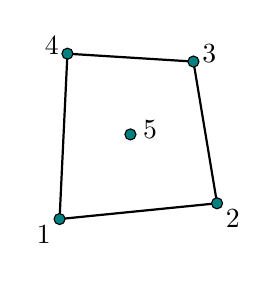
\begin{tikzpicture}
%\draw[fill=gray!23,gray!23](0,0) rectangle (5,5);
%\draw[step=0.5cm,gray,very thin] (0,0) grid (4,4); %background grid
\draw[thick] (1,1) -- (3,1.2) -- (2.7,3) -- (1.1,3.1) -- cycle;  
\node[] at (0.8,0.8) {1};
\node[] at (3.2,1) {2};
\node[] at (2.9,3.1) {3};
\node[] at (0.9,3.2) {4};
\node[] at (2.15,2.13) {5};
\draw[black,fill=teal] (1.9,2.075) circle (2pt);
\draw[black,fill=teal] (1,1)   circle (2pt);
\draw[black,fill=teal] (3,1.2)  circle (2pt);
\draw[black,fill=teal] (2.7,3)  circle (2pt);
\draw[black,fill=teal] (1.1,3.1) circle (2pt);
\end{tikzpicture}




Inside the reference element we assume that a field $f$
can be represented by 
\begin{eqnarray}
f^h(r,s) 
%&=& a+ br +cs +d \phi(r) +e \phi(s) \nn\\
&=& a+ br +cs +d \underbrace{\frac{5r^4-3r^2}{2}}_{\phi(r)}
+e \underbrace{\frac{5s^4-3s^2}{2}}_{\phi(s)} \nn
\end{eqnarray}
We then must have 
\begin{align}
f_1 &= f^h(r=1,s=0) &= a+ b +d \nn\\
f_2 &= f^h(r=0,s=1) &= a+ c +e \nn\\
f_3 &= f^h(r=-1,s=0) &= a- b +d \nn\\
f_4 &= f^h(r=0,s=-1) &= a -c +e \nn\\
f_5 &= f^h(r=0,s=0) &= a  \nn
\end{align}
and we easily get 
\[
a = f_5 
\qquad
f_1-f_3 = 2b
\qquad 
f_2-f_4 = 2c
\]
followed by
\[
d=f_1-a-b = f_1 - f_5 - \frac{1}{2}(f_1-f_3) = \frac{f_1-2f_5+f_3}{2}
\]
and 
\[
e = f_2-a-c = f_2 - f_5 -  \frac{1}{2}(f_2-f_4) = \frac{f_2 -2f_5+f_4 }{2}
\]
Finally:
\[
f(r,s) = 
f_5 +
\frac{1}{2}(f_1-f_3) r+
\frac{1}{2}(f_2-f_4) s+
\frac{f_1-2f_5+f_3}{2} \phi(r)+
\frac{f_2 -2f_5+f_4 }{2} \phi(s)
\]
i.e.
\[
f(r,s) = 
\left(\frac{r + \phi(r)}{2} \right)f_1 +
\left(\frac{s+\phi(s)}{2} \right)f_2 +
\left(-\frac{r-\phi(r)}{2} \right)f_3 +
\left(-\frac{s - \phi(s)}{2} \right)f_4 +
\left(1-\phi(r)-\phi(s) \right)f_5 
\]
which has us define 
\begin{eqnarray}
\bN_1(r,s) &=& \frac{r + \phi(r)}{2} \nn\\
\bN_2(r,s) &=& \frac{s+\phi(s)}{2} \nn\\
\bN_3(r,s) &=& -\frac{r-\phi(r)}{2} \nn\\
\bN_4(r,s) &=& -\frac{s - \phi(s)}{2}\nn\\
\bN_5(r,s) &=& 1-\phi(r)-\phi(s)\nn
\end{eqnarray}
We have of course the following properties $\sum\limits_{i=1}^5 \bN_i(r,s) = 1$ and 
$\bN_i(r_j,s_j) = \delta_{ij},\;  i,j \in 1,5$. 
The partial derivatives of the basis functions are as follows
\begin{eqnarray}
\partial_r \bN_1(r,s) &=& \frac{1 + \phi'(r)}{2} \nn\\
\partial_r \bN_2(r,s) &=& 0 \nn\\
\partial_r \bN_3(r,s) &=& -\frac{1-\phi'(r)}{2} \nn\\
\partial_r \bN_4(r,s) &=& 0 \nn\\
\partial_r \bN_5(r,s) &=& -\phi'(r) \nn\\
\partial_s \bN_1(r,s) &=& 0 \nn\\
\partial_s \bN_2(r,s) &=& \frac{1 + \phi'(s)}{2} \nn\\
\partial_s \bN_3(r,s) &=&  0 \nn\\
\partial_s \bN_4(r,s) &=& -\frac{1-\phi'(s)}{2} \nn\\
\partial_s \bN_5(r,s) &=& -\phi'(s) \nn
\end{eqnarray}
This element is implemented in the {\tt stone\_han.py} file in \stone~77 and also in \stone~120. 








%------------------------------------------------------------------
\subsection{The Divergence-free nonconforming $P_1^{NC}\times P_0$ pair} \label{ss:p1ncp0}



It belongs to the Crouzeix-Raviart family. 
The midside nodes are used as degrees of freedom for the velocities.
It is mentioned in Section~6.3 of \textcite{bobf08} (2008): ``[...]
It is exactly divergence free. Another important feature of this
element is that it can be seen as a "mass conservation" scheme. The present element
has been generalized to second order in \textcite{foso83} (1983).
It must also be said that coerciveness may be a problem for the $P_1^{NC} \times P_0$ 
element, as it does not satisfy the discrete version of Korn's inequality. 
This issue has been deeply investigated and clearly illustrated in \textcite{arno93} (1993).''

\begin{flushright} {\tiny {\color{gray} (tikz\_p1ncp0.tex)}} \end{flushright}
%~~~~~~~~~~~~~~~~~~~~~~~~~~~~~~~~~~~~~~~~~~~~~~~~~~~~~~~~~~~~~~~~~~~~~~~~~~~~~~~~~~~~~~~~~~~~~~~~~~


\begin{center}
\begin{tikzpicture}
%\draw[fill=gray!23,gray!23](0,0) rectangle (5,5);
%\draw[step=0.5cm,gray,very thin] (0,0) grid (5,3.5); %bckgr grid
\draw[thick] (1,0.5) -- (4,1)  -- (3,3) -- cycle; %1-9-2-6-5

%pressure nodes
\draw[violet] (2.75,1.5) circle (4pt); % 0 

%velocity nodes
\draw[black,fill=teal] (2.5,0.75) circle (2pt);
\draw[black,fill=teal] (2,1.75) circle (2pt);
\draw[black,fill=teal] (3.5,2) circle (2pt);

% legend
\draw[black,fill=teal] (3.1,0.2) circle (2pt); \node[] at (3.4,0.2) {$\vec\upnu$};
\draw[violet] (4.1,0.2) circle (4pt); 
\node[] at (4.4,0.2) {$p$};
\end{tikzpicture}\\
\end{center}



At page 170 of \cite{braess} it is stated that ``an analogous quadrilateral element was 
developed and studied by \textcite{ratu92} (1992)''.

In \textcite{bobf13} we find: ``We consider the classical (almost\footnote{What does that mean?!}) 
stable nonconforming triangular 
element introduced in \textcite{crra73}, in which mid-side nodes are used as degrees of 
freedom for the velocities. This generates
a piecewise linear nonconforming approximation; pressures are taken constant on
each element. It is also possible to build a three-dimensional
version of this element, using mid-face nodes as degrees of freedom.''
Also: ``It must also be recalled that coercivity is a problem for the $P_1^{NC}\times P_0$ 
element. The trouble is that the bilinear form (8.2.1) is not coercive on the 
nonconforming space $V_h$ and we do not have the discrete version of Korn's inequality.''

It is also mentioned in \textcite{john16}, appendix B.3, example B.43, in 2D and 3D, 
in \textcite{brfo} (example 8.1), and studied extensively in \textcite{john98} (1998). 

\begin{center}
\includegraphics[width=8cm]{images/pair_p1ncp0/john98}\\
{\captionfont Taken from \textcite{john98}.}
\end{center}

In \textcite{jolm17} (2017) the authors show results obtained with this element (fig 6) 
but also explain that these are obtained with so-called reconstructed test functions.
 


%------------------------------------------------------------------
\subsection{The Chen nonconforming ${ Q}_1\times Q_0$ pair (?)} \label{ss:chenq0}
\begin{flushright} {\tiny {\color{gray} \tt pair\_chen.tex}} \end{flushright}
%~~~~~~~~~~~~~~~~~~~~~~~~~~~~~~~~~~~~~~~~~~~~~~~~~~~~~~~~~~~~~~~~~~~~~~~~~~~~~~~~~~~~~~~~~~~~~~~~~~

What follows is tentative!

This space is proposed in \textcite{chen93b} (1993), albeit not in the 
context of the Stokes equations.

It is based on the mid-point variant of the RT basis functions, 
\begin{eqnarray}
\bN_1(r,s) &=& \frac{1}{4} (1-2s-(r^2-s^2)) \nonumber\\
\bN_2(r,s) &=& \frac{1}{4} (1+2r+(r^2-s^2)) \nonumber\\
\bN_3(r,s) &=& \frac{1}{4} (1+2s-(r^2-s^2)) \nonumber\\
\bN_4(r,s) &=& \frac{1}{4} (1-2r+(r^2-s^2)) \nonumber
\end{eqnarray}
to which a $P_2$ bubble is added
\[
\phi(r,s) = 1-\frac34(r^2+s^2)
\]
Note thath this function is zero at locations $\pm 1/\sqrt{3}$ 
on all four edges and exactly 1 in the middle. 

A field $f$ is represented inside the element by 
\[
f^h(r,s)=a \bN_1(r,s)
+b \bN_2(r,s)
+c \bN_3(r,s)
+d \bN_4(r,s)
+e \phi(r,s)
\]
We immediately see that this space is not interpolatory, i.e. the basis function $\phi(r,s)$ cannot be 1 in the middle and 0 at the other four nodes. 

\textcite{chen} also extends this to 3D in the paper. 

This space is used for velocity and a $Q_0$ space is used for 
pressure in \stone~120 (only because the basis functions above are
based on the Rannacher-Turek ones).


%----------------------------
\subsection{Other FE element pairs}

\begin{itemize}

\item ${\bm Q}_2\times Q_2$: This element is never used, probably because 
a) it is unstable, b) it is very costly. 
There is one reference to it in \textcite{hufb86} (1986).

\item ${\bm Q}_1\times P_{-1}$ Bilinear velocities,  piecewise linear discontinuous polynomial pressure.

\item See Fortin \cite{fort81} for various stable low order elements other than the enriched 
${\bm Q}_1^+ \times P_0$

\item ${\bm Q}_1\times Q_1$ + nonconforming null edge average \cite{fros07}

\item check \textcite{dhhu86} (1986) many flavours of triangles and quads.

\item Bercovier-Pironneau element pair, or $P_1isoP_2$.See \textcite{bocg12} (2012).

\end{itemize}

%.........................................................................
\subsection{A note about incompressibility and standard mixed methods}

What follows is nicely explained and demonstrated in John \etal \cite{jolm17}. In their 
example 1.1 they look at the velocity error of benchmark VJ2 (see Section~\ref{mms9}) 
which analytical solution is a zero velocity field. They show that for the MINI, 
Taylor-Hood and Crouzeix-Raviart triangular elements the velocity error grows 
with the magnitude of the rhs. They also make this statement:
``there are important applications, e.g., natural
convection problems, where the pressure is larger than the velocity by orders
of magnitude. In such situations, one cannot expect to compute accurate
velocity fields with classical mixed methods, at least for low order methods.''


